\documentclass[11pt,a4paper]{report}

% Aberstwyth dissertation LaTeX Template
% Authors: Dr. Hannah Dee (hmd1@aber.ac.uk), Neil Taylor (nst@aber.ac.uk)
% This has been adapted from the Leeds Thesis template and the 
% Group Project template for Computer Science in Aberystywth University.
% 
% All comments and suggestions welcome.
%
% Template designed to be used with pdflatex: it may need alteration to
% run with a different LaTeX engine

% To build document on the unix command line, run four commands:
 
% pdflatex dissertation
% bibtex dissertation
% pdflatex dissertation
% pdflatex dissertation

% you will end up with dissertation.pdf 
\usepackage{mmp}
\usepackage{graphicx}
\usepackage{pdfpages}
\usepackage{lscape}
\usepackage{cleveref}
\usepackage{listings}
\usepackage{subfig}
\let\citename\relax


% Things for javascript code inserts in document.....
\usepackage{color}
\definecolor{lightgray}{rgb}{.9,.9,.9}
\definecolor{darkgray}{rgb}{.4,.4,.4}
\definecolor{purple}{rgb}{0.65, 0.12, 0.82}

\lstdefinelanguage{JavaScript}{
  keywords={typeof, new, true, false, catch, function, return, null, catch, switch, var},
  keywordstyle=\color{blue}\textbf,
  ndkeywords={if, return, else, break, while, for},
  ndkeywordstyle=\color{purple}\textbf,
  identifierstyle=\color{black},
  sensitive=false,
  comment=[l]{//},
  morecomment=[s]{/*}{*/},
  commentstyle=\color{green}\ttfamily,
  stringstyle=\color{orange}\ttfamily,
  morestring=[b]',
  morestring=[b]"
}

\lstset{
   language=JavaScript,
   backgroundcolor=\color{lightgray},
   extendedchars=true,
   basicstyle=\footnotesize\ttfamily,
   showstringspaces=false,
   showspaces=false,
   numbers=left,
   numberstyle=\footnotesize,
   numbersep=9pt,
   tabsize=2,
   breaklines=true,
   showtabs=false,
   captionpos=b
}

% the following packages are used for citations - You only need to include one. 
%
% Use the cite package if you are using the numeric style (e.g. IEEEannot). 
% Use the natbib package if you are using the author-date style (e.g. authordate2annot). 
% Only use one of these and comment out the other one. 
\usepackage{cite}
%\usepackage{natbib}

% Use the following to selectively exclude chapters
%\includeonly{cover,abstract,acknowledge,declare,chapter1,chapter2}
\setlength\parindent{0pt}
\begin{document}

% all of the include directives below refer to tex files
% so \begin{titlepage}

\newcommand{\HRule}{\rule{\linewidth}{0.5mm}} % Defines a new command for the horizontal lines, change thickness here

\begin{center} % Center everything on the page


\includegraphics[scale=0.5]{images/logo.png}\\[0.6cm] % Include a department/university logo - this will require the graphicx packagecollege

\textsc{\Large Computer Science}\\[0.5cm] % Major heading such as course name

\HRule \\[0.4cm]
{ \huge \bfseries A WebGL-based aerobatic visualiser using the OLAN catalogue to provide a means of generating interactive 3D representations of manoeuvres. } % Title of your document
\HRule \\[0.6cm]

\huge{ CS39440 Major Project }\\[1cm]

\begin{minipage}{0.4\textwidth}
\begin{flushleft} \large
\emph{Author:}\\
Craig \textsc{Heptinstall} % Your name
\\ crh13@aber.ac.uk
\end{flushleft}
\end{minipage}
~
\begin{minipage}{0.4\textwidth}
\begin{flushright} \large
\emph{Supervisor:} \\
Prof. Neal \textsc{Snooke} % Supervisor's Name
\\ nns@aber.ac.uk
\end{flushright}
\end{minipage}\\[1.5cm]
{\large {7th May 2015}}\\ 
{\large {Version: 2.0 Release}}\\[1cm] 
{\large{This report was submitted as partial fulfillment of a MEng degree in Software Engineering (G601)}}\\[3.2cm]

\end{center}

{\large {Department of Computer Science}}\\ 
{\large {Aberystwyth University}}\\ 
{\large {Aberystwyth}}\\ 
{\large {Ceredigion}}\\ 
{\large {SY23 3DB}}\\ 
{\large {Wales, UK}}
\end{titlepage} includes cover.tex - to change the content,
% edit the tex file

\pagenumbering{roman}

% This is the front page
\begin{titlepage}

\newcommand{\HRule}{\rule{\linewidth}{0.5mm}} % Defines a new command for the horizontal lines, change thickness here

\begin{center} % Center everything on the page


\includegraphics[scale=0.5]{images/logo.png}\\[0.6cm] % Include a department/university logo - this will require the graphicx packagecollege

\textsc{\Large Computer Science}\\[0.5cm] % Major heading such as course name

\HRule \\[0.4cm]
{ \huge \bfseries A WebGL-based aerobatic visualiser using the OLAN catalogue to provide a means of generating interactive 3D representations of manoeuvres. } % Title of your document
\HRule \\[0.6cm]

\huge{ CS39440 Major Project }\\[1cm]

\begin{minipage}{0.4\textwidth}
\begin{flushleft} \large
\emph{Author:}\\
Craig \textsc{Heptinstall} % Your name
\\ crh13@aber.ac.uk
\end{flushleft}
\end{minipage}
~
\begin{minipage}{0.4\textwidth}
\begin{flushright} \large
\emph{Supervisor:} \\
Prof. Neal \textsc{Snooke} % Supervisor's Name
\\ nns@aber.ac.uk
\end{flushright}
\end{minipage}\\[1.5cm]
{\large {7th May 2015}}\\ 
{\large {Version: 2.0 Release}}\\[1cm] 
{\large{This report was submitted as partial fulfillment of a MEng degree in Software Engineering (G601)}}\\[3.2cm]

\end{center}

{\large {Department of Computer Science}}\\ 
{\large {Aberystwyth University}}\\ 
{\large {Aberystwyth}}\\ 
{\large {Ceredigion}}\\ 
{\large {SY23 3DB}}\\ 
{\large {Wales, UK}}
\end{titlepage}                        

% Set up page numbering
\pagestyle{empty}

% declarations of originality 
\thispagestyle{empty}

%%%
%%% You must sign the declaration of originality. 
%%%
\begin{center}
    {\LARGE\bf Declaration of originality}
\end{center}

In signing below, I confirm that:

\begin{itemize}
\item{This submission is my own work, except where clearly
indicated.  }

\item{I understand that there are severe penalties for plagiarism 
and other unfair practice, which can lead to loss of marks
or even the withholding of a degree. }
 
\item{I have read the sections on unfair practice in the Students' 
Examinations Handbook and the relevant sections of the 
current Student Handbook of the Department of Computer 
Science.}
 
\item{I understand and agree to abide by the University's
regulations governing these issues.}
\end{itemize}

\vspace{3em}
Signature ............................................................  \\

\vspace{1em}
Date ............................................................ \\

%%% 
%%% We would like to make a selection of final reports available to students that take 
%%% this module in future years. To enable us to do this, we require your consent. You 
%%% are not required that you do this, but if you do give your consent, then we will have 
%%% the option to select yours as one of a number of reports as examples for other 
%%% students. If you would like to give your consent, then please include the following 
%%% text and sign below. If you do not wish to give your consent, please remove this 
%%% from your report. 
%%%
\vspace{5em}
\begin{center}
    {\LARGE\bf Consent to share this work}
\end{center}

In signing below, I hereby agree to this dissertation being made available to other
students and academic staff of the Aberystwyth Computer Science Department.  

\vspace{3em}
Signature ............................................................  \\

\vspace{1em}
Date ............................................................ \\

               

\thispagestyle{empty}

\begin{center}
    {\LARGE\bf Acknowledgments}
\end{center}

I am grateful to some fellow students who provided help and support throughout this project, and for the numerous ideas they provided to me to assist with completing certain tasks. Ideas such as breaking down flight manoeuvres into a set of instructions were ones that were used to base my own design and implementation from. No code has been copied or taken and changed from another student. 

I would also like to thank the users who tested the completed application and who provided very vital and useful feedback. Feedback from these users was greatly appreciated and helpful when evaluating the application and project. The quick response to the questionnaires was also highly appreciated, due to the time constraints on the project.

Finally, I would like to thank my project supervisor. The clear sight of requirements has meant that it was possible to begin the project earlier than expected, giving me more time to work on important design and coding of the application. The request from the supervisor to create initial planning and research at the start of the project helped greatly in the overall analysis of the task, and a check-up of project progress mid-way through the project ensured I did not fall behind or have any substantial issues. % Acknowledgements
\thispagestyle{empty}

\begin{center}
{\LARGE\bf Abstract \& Background}
\end{center}

The aim of this project is to create a 3D representation of aerobatic manoeuvres, primarily using the OLAN notation(or one letter aerobatic notation). Both real-scale and remote control aerobatic planes and helicopters use the notation to describe a set of manoeuvres in an overall routine, usually including translating the notations into Aresti symbols. The Aresti symbols came before OLAN, but OLAN was developed to make it possible for pilots to write down quickly their planned routines.

The primary element of this project will involve allowing users to insert their notated routines into the application(via an input box on a web-page) thus producing first the ribbon shapes of the manoeuvres, followed by the ability to see a craft fly the route. Although there is only a finite amount of manoeuvres possible from the Aresti catalogue, each OLAN notation can have its own parameters. This can range from entry length into a loop or turn, to the number of rolls in a section of a manoeuvre. The application will also need to be taking into account flight speeds, and possibly wind and gravitational effects. The life cycle will be chosen after the initial list of requirements is apparant and in an orgaised manor.

WebGL will be the language used to create this application, with hopefully object-orientated Javascript to power the application. Libraries helping towards the graphical/ visual side of the application may be required to give greater flexibility and better aesthetic value. All considerations will be found in the analysis and design stages of this report.                 % Abstract

\pagenumbering{roman}
\pagestyle{fancy}
\fancyhead{}
\fancyfoot[C]{\thepage}
\renewcommand{\headrulewidth}{0 pt}
\renewcommand{\chaptermark}[1]{\markboth{#1}{}}

\tableofcontents   
\newpage
\listoffigures
\newpage 
\listoftables
\newpage

% Set up page numbering
\pagenumbering{arabic}

\setchapterheaderfooter

% include the chapters
\chapter{Background \& Objectives}
Before commencing the design of the application and the project planning, it is important to have analysed what I hope to have achieved at the end of my project time, and also what steps I will need to be taking to implement each feature. As I will mention later, using FDD will play a big part of how I shape my project and create each feature whether it be by priority, size or difficulty. This section details my understanding for my project requirements, steps I am going to need to take, and also the first sections of an FDD project; developing an overall model and building the list of requirements and features.

\section{Background}
The choice of undertaking a project such as this one was due to two combining factors: maths and an interest to learn graphical programming. The fact that this application will require me to learn graphics, and how to implement visual effects representing the requirements of the project in ways completely new to myself. As graphics is something I have not had much to do with in the past, this project appears both exciting and daunting task due to the learning curve I will need to take. As for the maths factor, I can assume quite a lot of maths will be involved(especially for creating curves, rolls and turns along most of the manoeuvres) which I enjoy learning about.\\   \\ \\
In terms of the background of OLAN and Aresti\\ \\ \\
Upon starting this project, several meetings with the project supervisor are planned each providing more detail of the initial requirements. Each of the meetings will be found in the Gantt for the project, with a smaller document in the\textbf{ appendix} showing the results of each meeting. Because I have already attended several meetings at this stage, I can provide a fairly accurate list of initial requirements of the application.\\

\noindent The initial required application can be broken down into an extensive(but less detailed) list of main functional requirements. These are as follows:
\begin{enumerate}
	\item Provide a web-implemented tool that: 1 that allows input of the OLAN 1 None-IE due to WebGL capabilities. Will it use a simple JSON file to store notations? characters as a string format, alongside possible click functionality.
	\item Relate each notation or set of notations to a certain procedural
movement2 (rotations, movements etc.). 2 Must consider parameters in some of
the notations, such as the speed of entry
	\item Provide a means of linking up these movements in such a way into moves, or the angle of the plane.
they produce a fluid manoeuvre.
	\item Display this using WebGL3. Libraries4 to consider that could help 3 Begin by initially testing simple shapes
to move and fly around, then add
textures, and plane strcture.
	\item Are libraries ok to use?
with some of the movements:
• glMatrix- Javascript library for helping with performing actions
to matrices- http://glmatrix.net
• ThreeJS- Another Javascript library, good with handling cameras
and different views- http://threejs.org
	\item Allow user to add different effects such as wind, gravity changes
and other physics5. 5 Could be better to implement these
last, as it will be easier to test pure
functionality of rolls etc first, then
figure out natural physics.
	\item Add functionalities of different viewpoints(on-board views, side
views) to application.
	\item Possibility to add function to save (using local storage?) users
different sets of manoeuvres?
\end{enumerate}
%Taking into account the problem and what you learned from the background work, what was your analysis of the problem? How did your analysis help to decompose the problem into the main tasks that you would undertake? Were there alternative approaches? Why did you choose one approach compared to the alternatives? There should be a clear statement of the objectives of the work, which you will evaluate at the end of the work. In most cases, the agreed objectives or requirements will be the result of a compromise between what would ideally have been produced and what was felt to be possible in the time available. A discussion of the process of arriving at the final list is usually appropriate.

\section{Analysis}


\section{Process}
%You need to describe briefly the life cycle model or research method that you used. You do not need to write about all of the different process models that you are aware of. Focus on the process model that you have used. It is possible that you needed to adapt an existing process model to suit your project; clearly identify what you used and how you adapted it for your needs.


%\addcontentsline{toc}{chapter}{Development Process}
\chapter{Design}
On completion of my analysis and background planning for the project, I can now look at more detailed design for the application overview, and the individual component it comprises of. Becuase my application will present both a front-end GUI and back-end Javascript and WebGl, I will split my design into two sections. The reasoning for this is becuase I would prefer to have the GUI and logic of the application to be decoupled, so that the code can be changed in the Javascript easily without having to affect the user interface. Other than planning the application itself, it is also important I plan what key assisting services I use, such as how I intend on versioning my code, to how I will deploy my code.

\section{Overall Architecture}
As a summary of the architecture of my planned application, the best way to design in more detail is to lay out a primary design pattern. For the purpose of an application which will allow for user interaction, which will be processed by code in the back-end, I have decided to go ahead with a Model-view-controller approach. Using the MVC pattern means I can separate the GUI from the logic code as I wanted to, and have the GUI exists without knowledge of the back-end. This is also the same with the model, where the primary code for calculating manoeuvre movements and animations should be possible without knowledge of the view, but instead use the controller as a intermediary. See figure ~\ref{fig:mvc} for the MVC pattern I plan to use. 

\begin{figure}[h!]
  \centering
      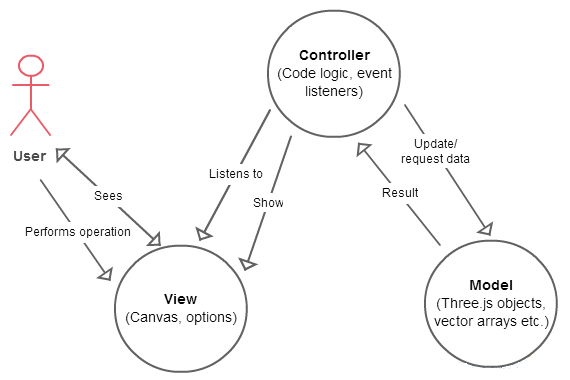
\includegraphics[width=0.8\textwidth]{images/mvc.png}
  \caption{Model View Controller diagram for my proposed application. Shows the planned interactions between different subjects within my application.}
  \label{fig:mvc}
\end{figure}

Because I have already chosen three.js as library of choice for creating any graphics and physics objects, these will already form my model or models. Each manoeuvre for instance will be reflected as a set of vectors which will form the shapes of the Aresti flight paths, and should be accessible and changeable through the controller to the view(in this case the canvas in my GUI).

The controller will be the most crucial part I implement, as it will need to be able to communicate with the three.js objects, the canvas disaplaying the animation, and detect controls from the user. For this piece of the pattern, I will enforce some other design patterns to 

Finally, the view will be represented as the canvas and controls on the web page. Since on both the canvas and the options menu can have an affect on the model, the controller will listen for changes on either, and then call the relevent operations to affect the model, and again reflect this back onto the view. The view will not know anything of the controller nor the model, so adding any new options or displayable information will be easier and not conflict with any current elements.

\section{Back-end logic and design}
The first of the two design categories concentrates on the JavaScript that will act as the functions to run each of the proposed features of the application. The code on this side will be responsible for maintaining contact with the GUI, and more importantly the WebGL canvas on the web page. To make the code be as maintainable and run effectively as possible, I will look into a variety of design patterns.

\subsection{Design patterns}
Because I am using a hybrid of waterfall and FDD at this stage of the project, using a changing range of design patterns for my JavaScript and GUI architecture is possible. Through the implimentation stage of this report, some of these may patterns mentioned may not be used anymore and replaced for different ones depending on changing requirements and progress. Using the implement, refactor and test iteration approach should allow for this.

The first design pattern that would be good useful relating to the controller is known as an observer pattern. The observer pattern means to listen on an event or events in an application, and then call the relevent action. The JQuery library, which I plan to use throughout any GUI related tasks will be of a great use here. This library will allow me to add simple listeners on elements on the web page, and set methods to be called on any click, hover or other events. In terms of how I will place this pattern in my archetecture, a standalone file will be responsible for listening to any options or menu changes, whilst another JavaScript file will be repsonsible for listening to the canvas events such as rotation or zoom.

The next design pattern I plan on implementing into my application relates again to the MVC archetecture I will be using. The builder pattern will allow me to append and edit any HTML on the page(such as options, checkboxes, loading content back into the OLAN input box) easily with data retreieved from the model. JQuery again should help to provide a means of changing content, becuase of more built-in method it comes with. There should be a handler class in my application specifically for controlling the page content.

A third design pattern which will be important when it comes to loading up the application will ensure that all the data nessecary to run the application is ready before the user can perform any actions. Known as the Lazy initialisation pattern, this is a style of coding that means whenever files or data is being loaded, the rest of the application should either wait, or prevent other relying features from being initialised. One motivation for the need for this pattern in my program is becuase of the vast amount of manoeuvre data, and model data for terrain or for aircrafts means that functionality such as animating and drawing flight paths on the canvas may be already ready for use from the user before all the data is ready. In this case, it could cause errors and even crash the application. Therefore, making sure that the application does not progress loading before data is ready is of great importance.

Although the previous design patterns have been chosen, others were considered when planning the application but were not suitible or better options were availible. One such pattern, the Mixin pattern allows JavaScript functions to be inherited from other classes or inner functions. For instance, these would be useful as a means of decreasing repition of functions. In my proposed application, I thoguht about the possibility of using a Mixin style architecture to allow functions that would draw both the manouevres on the canvas, and the manoeuvres on the movie-reel. The reason I have decided not to use this pattern falls to the issue that by making an object extend and hold code from elsewhere could make it harder to maintain, see where the function comes from, and uncertainty of location of any bugs I may come across while developing.

\subsection{Module diagram}
Because much of the code I will be implementing will hold various Three.Js objects, I have decided that modulating methods and objects will be better than simulating classes seeing as JavaScript is a class-less language. This is a pattern known as the module pattern. Although this may appear less object orientated, modules allow for more robust archetecture where units of code can be separated and organised. Modules are slightly similar to classes in the way they can hide code that should not be accessable to other modules by encapsulates privacy. When code is modulated, and then that module is called upon by another, only a public API is returned, and other methods in that module are kept private from being used in other parts of the application. These private methods are good for use as supporting methods, holding such things as calculations, or private variables for getters and setters. Again, this is a similar case to the traditional class diagram.

There are currently a selection of libraries that allow for modules in JavaScript. The most promininent, and the one I would like to use is called RequireJS, which promises the increase in speed and quality of code. RequireJS works by dynamically loading JavaScript files on the fly, where the code has from the other module is usable once loaded into the module calling it. Once modules are loaded into an object form in whatever the developer needs to name it, its public variables and methods can then be accessed. See figure ~\ref{fig:module} on how modules are used. In my case, modules would be useful in enforcing the MVC pattern in the way that it will help towards hiding code between the view and the model. 

\lstset{language=JavaScript}
\medskip
\begin{lstlisting}[caption=Example showing how RequireJS loads in another module or Javascript file which in this case is loading up the util javascript module and naming it as object 'util' for use in the code]
require(["helper/util"], function(util) { 
	
	// This function can not be called by another module
	function private_function(){
		util.Method() // Can call public methods in the util file
	}
	return {
		public_function: function(){
			// can be called if this module is loaded into another
		}
	}
});
\end{lstlisting}
\label{fig:module}

In order to create a basis for modulating code, I should first look to seperate the features I listed in the analysis section of this report into categories. These categories will then help me to determine how I could structure my application in as best object orientated way as possible.

The categories I have been able to come to are:
\begin{itemize}
  \item Main- initiating other modules, beginning the application.
  \item Animation- Playing, and controlling speed, physics of animation.
  \item Loading manoeuvres at start of application.
  \item Saving and loading animations
  \item Cameras- Creating and controlling cameras movements
  \item GUI controlling- control and edit GUI controls, and appearence from back-end. Also including the possible movie reel live animatiion.
  \item Canvas controls- Allowing the user to move along the canvas, and zoom.
\end{itemize}

Now I have a stable list of categoried features, I am able to create a diagram shown in figure ~\ref{fig:mod} to represent what modulated layout my applicatioon will use. Becuase of the way modules handle public and private variables, have public and have private methods, means that this is very reminiscent of a standard class diagram.

\begin{figure}[h!]
  \centering
      %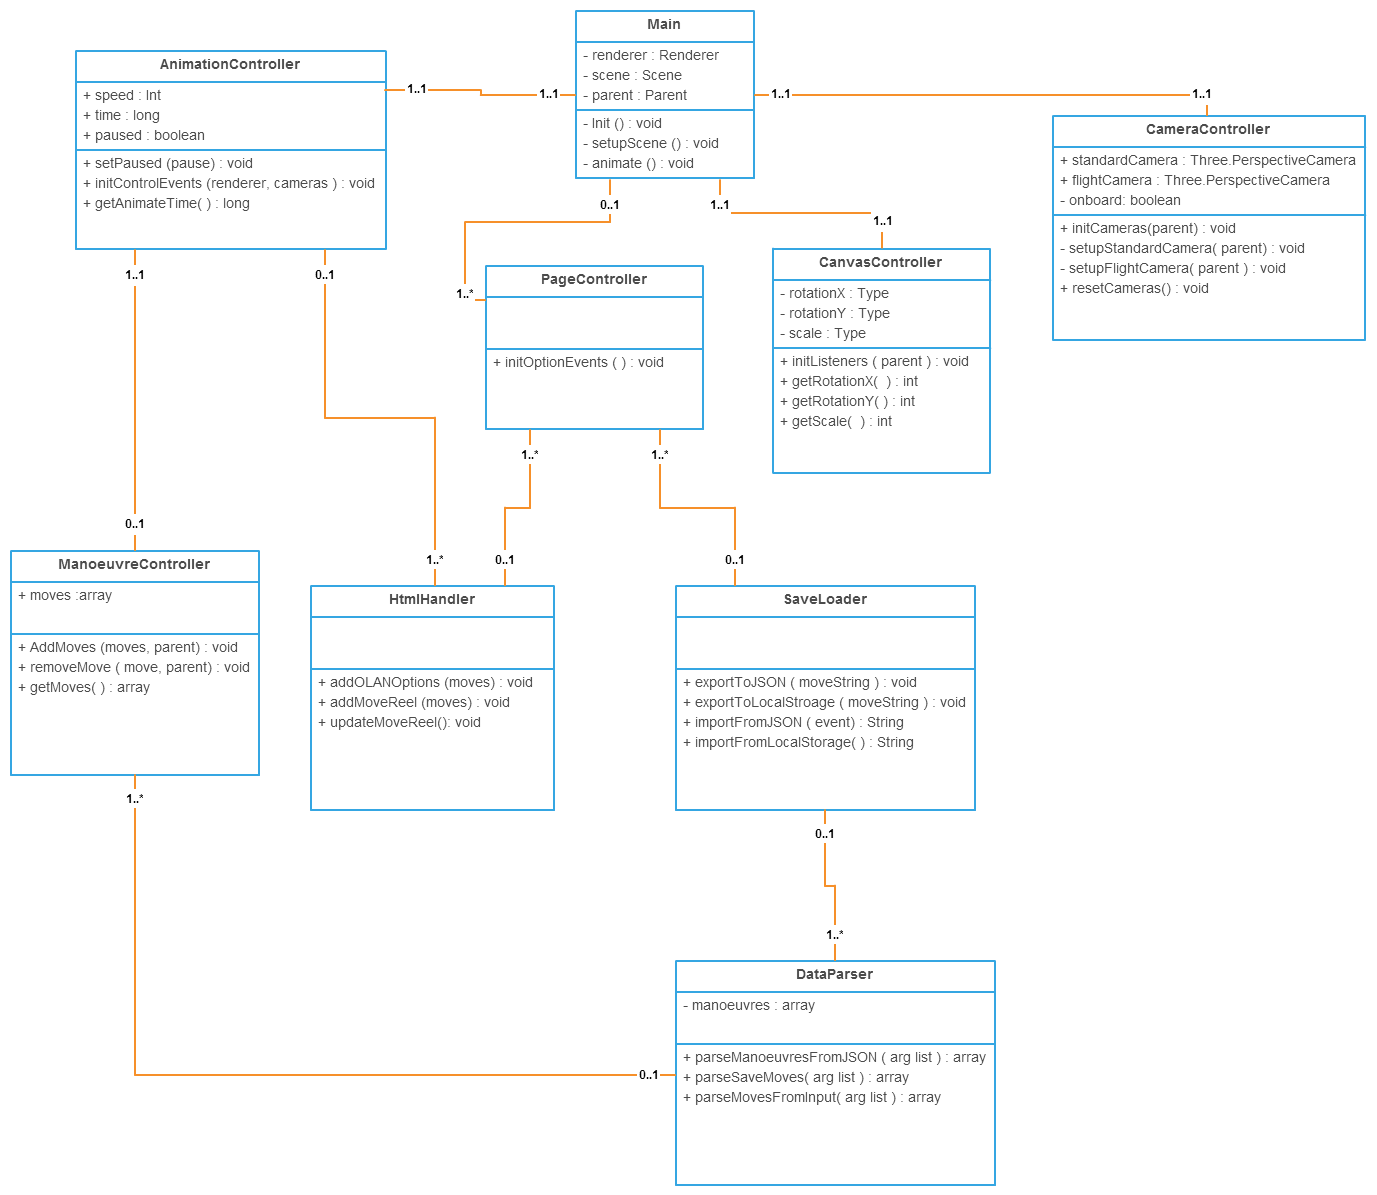
\includegraphics[width=0.8\textwidth]{images/mod.png}
  \caption{Module diagram displaying the various communications between modules, and how they are connected to the GUI in the MVC way.}
  \label{fig:mod}
\end{figure}

This module diagram shows what will be the communications between modules in the application, providing insight into what each module should contain in terms of important variables and methods. Ensuring that only modules that require certain peices of information from another module has sole access is important to reinforce the module pattern mentioned earlier. It should be noted here that although the diagram shows the main modules that will oversee most of the features of the application, when implementation occurs later on in the project, more modules or JavaScript files may be added to support or lighten the load of functions. This is supported by the good practice of \textbf{keeping files and functions short and concise} for easier maintenence and readability. The following descriptions have been kept brief, and key connections within the diagram discussed.

The first module propsed from the diagram will be the module entitled 'Main', which will be responsible for setting up the application, and hold onto key variables such as the renderer and scene objects to allow for anything to be drawn and animated on the canvas. This module will be called from the HTML and then will begin any nessecary calls to set up the listeners for the cameras, canvas and options. The most importat call will be the call to set up the animation controller module. 

Following on, the animation controller module will be one of the largest and most important parts of the overall architecture, as it will be responsible for both animating flight paths, loading up the OLAN manoeuvres at start of the application, and relating any actions from the user to do with OLAN selections or playing and pausing, as well as chaning animatiton speeds. 

The animation controller module will be in communication with the manoeuvre controller, which will be a logic heavy class because of the calculations it will require to compute and construct the sets of vectors of the Aresti shapes representing each OLAN notation. As the diagram shows, the application will first get the user OLAN input from the webpage via the HTML handler module, then search via the dataParse module and create the manoeuvres array object within the manoeuvre controller holding all the calculated manoeuvres, and return this in a 'get' method to the animation module for placing on the canvas.

As mentioned earlier, the HTML handler module will be the first means of contact to the user of the application, retreving input from the OLAN box, getting values of any checkboxes, and also setting any values. This module will be using the JQuery library as well as the Handlbars library as the primary way to communicate with the front-end, by diectly referencing ID's of divs on the webpage.

Two other controllers that should be mentioned are the camera dna canvas modules. Both modules will be resposible for setting up their elements when the applicaton starts up (including the different sets of cameras, locations, lighting and ground effects) and for listening to evens on both of their respective related front-end sections. Whilst the canvas module will only need to listen for events on the canvas and then reflect this by modifying the canvas directly, the camera controller will need to communicate with the manoeuvre module if the user is using the on-board view to get the current location on the flight path and then place the camera there. 

The final module to be highlighted in the diagram is the save and loading module, responsible for the storage of user input and flight paths. Becuase I suggested two means of saving flight paths, through JSON and through Local storage % FINISH HERRRRRRRRRRRRRRRRRRRRRRR

\subsection{Object and storage formatting}
It is imperative that the structure of data, espeically the OLAN instructions for construction of each manoeuvre is organised effiecently and be as accessable as possible, to consider the speed of the application running in a user's browser. 

\subsection{Naming conventions}


\section{User Interface}

\subsection{GUI Use-case}

\subsection{CSS and wireframe design}

\section{Planned use of services}

%You should concentrate on the more important aspects of the design. It is essential that an overview is presented before going into detail. As well as describing the design adopted it must also explain what other designs were considered and why they were rejected.The design should describe what you expected to do, and might also explain areas that you had to revise after some investigation.Typically, for an object-oriented design, the discussion will focus on the choice of objects and classes and the allocation of methods to classes. The use made of reusable components should be described and their source referenced. Particularly important decisions concerning data structures usually affect the architecture of a system and so should be described here.How much material you include on detailed design and implementation will depend very much on the nature of the project. It should not be padded out. Think about the significant aspects of your system. For example, describe the design of the user interface if it is a critical aspect of your system, or provide detail about methods and data structures that are not trivial. Do not spend time on long lists of trivial items and repetitive descriptions. If in doubt about what is appropriate, speak to your supervisor. You should also identify any support tools that you used. You should discuss your choice of implementation tools - programming language, compilers, database management system, program development environment, etc.Some example sub-sections may be as follows, but the specific sections are for you to define.

\chapter{Implementation \& Testing}
Following from the analysis and design of the application, it is now possible to start implementing the features produced from investigating the requirements earlier in the project. As it was already stated that the project would be running under an FDD means, rather than having two sections (one for implementation and one for testing), this section will show each feature one-by-one. By following this scheme, the feature prioirty list will be utalised to ensure the more important features are done first, and that they fulfil their function before moving on. However, this should not hide the fact that issues are possible when implementing and any such issues could hamper further development. If this does occur, the issues and reasons will be explained, followed by what judgement was made to continue on with development of the application as a whole.

\section{FDD project approach}
As mentioned, the feature driven development methodolodgy will now shape the approach that is taken to create each feature. Although design has already been completed for all features, there are still elements to each iteration that should be outlined before proceeding. The best way to plan this is to give a brief list of steps that will be performed in each iteration. This is as follows:

\begin{enumerate}
\item Give a re-cap on the requirements of the feature
\item Provide a walkthrough of implementation (with code samples)
\item Show tests used (JSUnit, usability tests) and results
\item Describe and differences with the feature and original design
\item If there are any issues, describe and give explanations
\item Give a progress log on the item, and provide dates and length of completion for use in accordance with the Gantt chart originally constructed
\end{enumerate}

It should also be noted that once the duration of the time in the project for the implemtation and testing stage is complete, a burn down and progress report will be possible to generate and will be done so. This will give a good idea of exactly the status of the project (with a calculated percentage), to see how much work was done compared to estimates, and to find out how succesful the project was overall. 

\subsection{Iterative Implimentation}
Before the iterations begin, it should be mentioned that although the order of features to be implemented were decided in the analysis, in order to impliment any back end things and allow for proper testing (usability testing), some basic GUI must be created first. Becuase of this, this will be the first iteration, followed by creation of the JSON manoeuvres. Following these iterations, it will then be much easier to test future features created. Without a basic GUI and canvas, it will be impossible to see the effects created whilst adding features such as drawing flight paths or moving cameras. After these two moved features are complete, the prioritised list will run as planned initially.

\subsubsection{Feature 1- Create a basic GUI}
The first feature that was to be implemented was less of a feature but more a requirement so the other features could be then created. The GUI or front-end of the application is important to be created, otherwise testing future WebGL features will not be possible. The requirements of the front end were:

\begin{itemize}
\item A responsive front-end that is mobile compatible
\item Have hidden menus that can push in from the left
\item Have basic inputs such as the OLAN input, and menu options
\item Provide a help and about page that overlays the application web page
\end{itemize}

The first task that was performed to create this task was to create a minimulistic layout matching the wireframes designed in chapter 2 of this report. The first action performed was to get the latest Foundation \cite{foundation} css library file, and then to create a layout using the features from the library. The navigation was made using the 'navbar' markup, which helps stick the navbar to the top of the page, alongside automatically changing into a mobile pull down menu once the screen size reaches a certain amount. Then using other mark-ups provided by Foundation I was able to float the various navigation bar buttons to their respective sides. 

The most important part of the GUI which has now been implimented is the off-canvas feature menus. The code for this can be seen in section~\ref{code:canvas} of appendix C. The way that Foundation helps create this off cnvas option is by wrapping everything in one div, then seperating the menu and content in half. When a user then pushes the designated button with the wrapper id, the entirety of the wrapper is pushed to the right to display the menu and less of the content. The about and help pages were also added successfully, with the addition of another library called Modernizer. This library allowed for a clean effect to overlay the information on top of the webpage.

Once the basic HTML elements with relevent ID tags were added to the index page of the application, it was then possible to add some custom style to the page. As mentioned in the design stage, it was possible to download Foundation modified with the colour scheme designed for the application. Changing backgrounds to black and text to white was very easy, and then added to the site. The colour and design of the page can be seen below in figure~\ref{fig:newgui}.

\begin{figure}[h]
  \centering
      %\includegraphics[width=1\textwidth]{images/newgui.png}
  \caption{Screenshot of GUI created with Foundation, JQyery and HTML markup.}
  \label{fig:mod}
\end{figure}

As planned, Sass was used to style specific elements of the page, such as the width of the OLAN input box, and to change text placement on the help and about pages. Setting up the Sass with Koala was easy, and upon each save of the file, CSS was compiled. 

One final mention goes to the creation of the WebGL canvas. To create the basic canvas, only a few lines of JavaScript was needed. To create it, a renderer was created using  the 'THREE.WebGLRenderer' object. Becuase this is early in the implementation stage, it was created without RequireJS as the archetcure is only one JS file. Once the object is created, JQuery appends the '.domElement' of this object to the container div created in the basic HTML. For future features, the WebGLRenderer object with be where any objects such as flight paths are added to.

As for testing this feature, becuase very little JavaScript was required to be coded here, usability testing was the only way to check for the completion of what was required. The test results can be found in Appendix D under section~\ref{test:canvas}. Overall, this feature has been made to 100\% of the requirements laid out, and matches the deisgn very well. Therefore, the progress tracker for this feature can be shown as:

\begin{table}[h]
\begin{tabular}{|l|l|l|l|p{7cm}|}
\hline
\textbf{Start} & \textbf{End} & \textbf{Duration} & \textbf{Progress} & \textbf{Comments}                                                                                                     \\ \hline
09-03-2015     & 10-03-2015   & 2 Days            & 100\%             & Complete, though once new features are under way, RequireJS will be utalised and the WebGL Canvas code will be moved. \\ \hline
11-03-2015     & 11-03-2015   & 1 Day            & 100\%             & Testing complete, usability table created and tested on mobile and desktop devices.\\ \hline
\end{tabular}
\end{table}

\textbf{Feature overall progress: 100\%}

\subsubsection{Feature 2- Convert OLAN and Aresti to JSON form}
The second feature, which was of high importance to the rest of the application was to create OLAN interpreted JSON which would give instrctions on how to construct each manoeuvre. Becuase this was quite thoughroughly planned and then designed how each instruction was going to broken down, the time designated for this task felt generous. Simply using the template created in the design, it was possible to fill in each instrction part by part through each OLAN manoeuvre. An example of some instructions can be seen in Appendix C in section~\ref{code:jsonmoves}.

The only time consuming part of this feature was the shear amount of different manoeuvres that had to be converted. For this reason, not every OLAN letter was created. The reason for this is becuase some moves are possible to be created from others, so further in development, more will be possible to be added. 

To support this feature, more JavaScript code had to be added to allow the JSON to be read into an object to begin drawing moves onto the canvas. Becuase the code would be in a different module to the WebGL canvas that was created in the previous feature, RequireJS now had to be added to the source code. To do this, the RequireJS library was added and initiated in the HTML page of the application as shown here in Appendix C section~\ref{code:requireJS}. Then a new module was created, named 'Dataparser' as designated in the design. The method for converting the JSON can also be found in the data parser module shown again in the appendix under section~\ref{code:jsonmovesJS}.

Once the coding and converting to JSON was complete, testing the code that performed the conversion to an object was required. By using JSUnit, it was possible to call the method that was created to instantiate the manoeuvres array, and pass in some raw JSON string, then compare to what the result should be. The JSUnit code can be found in appendix D, section~\ref{test:jsonmvoes}.

Like the last feature, no changes from the original design were performed, resulting in a good standing of time compared to the Gantt chart for the project. The feature progress can be expressed as percentages and final comments added again.

\begin{table}[h]
\begin{tabular}{|l|l|l|l|p{7cm}|}
\hline
\textbf{Start} & \textbf{End} & \textbf{Duration} & \textbf{Progress} & \textbf{Comments}                                                                                                     \\ \hline
12-03-2015     & 16-03-2015   & 5 Days            & 80\%             & JSON created to represent most manoeuvres, for that reason it is not an exact 100\& progress. JavaScript code and RequirejS functionality added to support the rest of the application. \\ \hline
17-03-2015     & 18-03-2015   & 2 Days            & 100\%             & JSUnit tests created and passed successfully, showing JSON matches up with manouvre array object.\\ \hline
\end{tabular}
\end{table}

\textbf{Feature overall progress: 90\%}

\subsubsection{Feature 3- Creating a scene with terrain and lighting}
The third feature, which is another to be brought forward ahead of flight path creation is the terrain and lighting effects. The reason for creating this before the OLAN construction is the same as creating the canvas, becuase without an area to see where the paths are drawn onto, the effects of that feature will be hard to test if it is working. Especially terrain, where the need for this is to see where the X axis of 0 will be. Without this, when implementing checks such as if the path would hit the ground would be harder to test. Again, the three.js library was of great use here, especially with built in methods to allow for lighting to be added.

In order to have started this feature, another module was added to the archetecture named 'TerrainHandler', which was where both lighting and ground was to then have their methods of adding to the canvas. This feature was found to be the shortest of the features, as it only required two simple methods. Rather than passing the renderer canvas object to this module to add the ground and lighting, it was decided to simply make both methods like factories to return the ground and lighting objects to where they were called from. In the case of where this module was called from, the main class where the canvas was created seemed the best place to call each method, as everything to do with setting up the scene could remain together and be easily understood or developed further.

As for testing, by keeping the terrain and lighting in their own module also helped towards testing the new methods. Two very simple tests were made using JSUnit to check the returns of each method, and both were added to the Jasmine instructions under each Github commit through the Travis builds. As with other tests, the test cases can be found in the appendices under appendix D section~\ref{test:lights}. This feature was fairly straight forward to implement and test with help from the three.js documentation site, therefore teh feature was done in less time than originally planned.

\begin{table}[h]
\begin{tabular}{|l|l|l|l|p{7cm}|}
\hline
\textbf{Start} & \textbf{End} & \textbf{Duration} & \textbf{Progress} & \textbf{Comments}                                                                                                     \\ \hline
19-03-2015     & 20-03-2015   & 1 Day            & 100\%             &  Completed module for terrain and lighting, linked up to main module.\\ \hline
20-03-2015     & 20-03-2015   & 1 Day            & 100\%             &  Two JSUnit tests created, and passing successfully.\\ \hline
\end{tabular}
\end{table}

\textbf{Feature overall progress: 100\%}

\subsubsection{Feature 4- Cameras}
The final predessing feature before the creation of OLAN paths that was decided should be ready were the various cameras that will look around the canvas. The initial requirements for cameras was to have two different views: one for navigating around the canvas, and the other for being onboard the flight path. At this stage of the project, creating the second was only possible to a certain extent, becuase without the construction of the paths yet, getting the location of where the onboard camera should be is not possible. Therefore, for this requirement both cameras were created, with the exception of the onboard camera where functionality is currently restricted. 

To start, another module was created for the 'CameraController'. Becuase it was best to keep the cameras completely seperated from other parts of the application to reduce decoupling, both camera objects were stored in this module and provided get and set methods for calls from other modules. An inititiator method was created for use from the main module, to create both camera objects at start up. Both these objects were again availible from the three.js library as 'THREE.PerspectiveCamera'. Then by passing the module around to any other modules, it will then be possible to update and retreive each camera object again. Alongside the camera creation, a controller for changing the angle of view, zoom and co-ordiantes was created as another module. 

This module, which has been called 'CanvasController' as designed in the module diagram, adds event listeners for dragging the mouse around the canvas, keyboard presses to move up and down, and scroll for zooming. Then by getting the new updated values of view-point angles, these are passed back to the camera controller which updates the values of each camera. By repeating this in a render loop in the main module, the updating of cameras is done several times a second, to make movements appear fluid. To help this, the code was refeactored several times to ensure that the amount of work done by the browser is as little as possible on each loop of the animation.

As for testing, alike the first feature where usability testing was the primary and sole means of checking the implementation fulfills the feature, JSUnit testing was not used. Usability testing was found the best option here, and results can be found in appendix D section~\ref{test:cameras}. During testing, it was found that there was an issue that when rotating the camera around the canvas, it seemed to always rotate around the point (0,0,0). This meant that navigating the canvas was slightly harder than it should have been. This was fixed though, by simply moving the camera rather than the scene in the canvas. As for the camera that was designed to be as on board view, a model airplane was added to represent the camera so it could be seen on the canvas. Although it does not move yet, the plane loads up at the start of the application and can be placed anywhere on the scene. You can see the plan on the canvas at point (0,0,0) below in figure~\ref{fig:plane}. The plane model is constrcuted from a JSON file from a page on the web with thousands of free models.

\clearpage

\begin{figure}[h!]
  \centering
      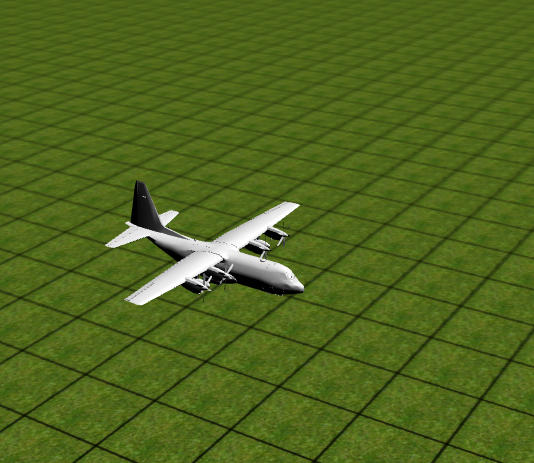
\includegraphics[width=0.6\textwidth]{images/plane.png}
  \caption{Model of plane loaded up using JSON and three.js object loader. This plane will represent the onboard camera, and fill be the object that will be assigned locations along an OLAN path to show flying the flight plans entered by users.}
  \label{fig:plane}
\end{figure}

The progress of the task is shown below. This feature was done exactly to its requirements in the design, and the modulation of code is still being followed.

\begin{table}[h]
\begin{tabular}{|l|l|l|l|p{7cm}|}
\hline
\textbf{Start} & \textbf{End} & \textbf{Duration} & \textbf{Progress} & \textbf{Comments}                                                                                                     \\ \hline
21-03-2015     & 23-03-2015   & 3 Days            & 100\%             &  Both cameras now usable, with constructer methods, and update methods. On board camera ready but not linkable to rest of application until animation of flight paths is ready.\\ \hline
24-03-2015     & 24-03-2015   & 1 Day            & 100\%             &  Usability tests complete, one change made to code following a failed test. \\ \hline
\end{tabular}
\end{table}

\textbf{Feature overall progress: 100\%}

\subsubsection{Feature 5- Construction of 3D paths from OLAN}
The most important feature, drawing shapes onto the canvas using the instrctions read in from JSON files was next to be implemented. The main requirement here was to draw smooth shapes that match the Aresti shapes as accuratly as possible, also bearing in mind that they should be linkable.

Using the array of maneouvre objects inported from JSON in the first feature implemented, creating shapes based on these was a matter of building up an array of vectors with each new vector being copied from the previous and then having the next instruction take effect on it. To do this, under a new module 'ManouevreController', a method was created that firstly found whih manouvre was to be built, then loop through the instructions of that manouevre creating it vector-by-vector. An example of how vectors were calculated is shown below in figure~\ref{fig:vectors}.

\begin{figure}[h]
  \centering
      %\includegraphics[width=1\textwidth]{images/vectors.png}
  \caption{Flow chart of how vectors were used to construct the spline shape.}
  \label{fig:vectors}
\end{figure}

As you can see, once vectors were created, they were passed to a three.js object which was a spline curve. A spline curve is one that interpolates along all its points to create a smooth shape. Once points are added to this object, it can then be added to the canvas. Upon initial usability testing of this, it was found that many of the joins between points were well-off center, due to the interpolation being too large. This was down to the fact that with each turn instruction being a 45 degree angle, meant that the change was too sharp from a straight to curved line, so the straight line was affected too much. To fix this, by dividing up the 45 degree into smaller pieces meant that interpolation was needed much less, therefore the curves appeared smoother and had much less effect on any predecessing straight lines.

Another big issue that appeared during testing was that any manoeuvres that had a change in angle through a turn always seemed to revert back to a straight line, meaning the rest of the manoeuvre was out of sync and did not look correct. This was an especially time-consuming bug, and a example of it can be seen in figure~\ref{fig:issue}. Becuase finding out the problem and attempting to fix it was eating away at other feature time, the issue was left for the time being, in order to complete other key features outlined in the requirments. In order to ensure this issue would not remain at the end of the project, a strict time limit was set on the next features to allow for a good amount of time to fix the issue here.

\begin{figure}[h]
  \centering
      %\includegraphics[width=1\textwidth]{images/vectors.png}
  \caption{Flow chart of how vectors were used to construct the spline shape.}
  \label{fig:vectors}
\end{figure}

At the end of the iterations in this report, this issue will be re-evaluated once the fix is in place. Other than this issue, the rest of the feature was implemented well, and entering OLAN now drew fairly accurate shapes. Again with testing, usability was the primary case here, becuase checking for correct spline curves created would be too time consuming and difficult with the use of JSUnit. The overall progress of the task at this point of the project is as follows:

\begin{table}[h]
\begin{tabular}{|l|l|l|l|p{7cm}|}
\hline
\textbf{Start} & \textbf{End} & \textbf{Duration} & \textbf{Progress} & \textbf{Comments}                                                                                                     \\ \hline
25-03-2015     & 05-04-2015   & 2 Weeks            & 75\%             &  Although OLAN now is represnted by shapes and they link up correctly, the issue mentioned os straight lines being drawn on change of angle remains. This will be fixed fully after implementtaion of other tasks.\\ \hline
06-03-2015     & 08-03-2015   & 2 Days            & 75\%             &  Usability tests complete, changed step of angles from 45 to 15 to get smoother interpolation. More tests will be required after fixing the issue.\\ \hline
\end{tabular}
\end{table}

\textbf{Feature overall progress: 75\%}

\subsubsection{Feature 6- Animate OLAN flight path}
Although there was an issue imnplementing the drawing of flight paths in the previous feature, the functionality that was complete allowed for the animation feature to be done. Three.js provided a good means of getting points along the spline curves to a percentage of the length of the shape. For example, by using the method 'getPointAt' with 50 as the paramter value gave the return vector value of the point on the line halfway. By doing this iterativly using the render loop used in the cameras meant a value could be incremented over time, thus getting points along each curve. Each time a point was received, the on-board camera could then be set to the position of it, and by doing this as fast as the render loop meant that a smooth animation was created. Again, a new module was created 'AnimationController' with various methods for playing and pausing the animation, and setting the distance of time between each point recieved in order to speed up or slow down the animation.

With each curve being stored in an array object, meant if linked up manoeuvres were being animated along, once one manoeuvre had reach 100\% for getting points along its line, the next manoeuvre would be selected from the array and the get-point percentage reset back to 0. By doing this, a flawless smooth cross between manoeuvres has been achieved.

As for testing this feature, more JSUnit was used, but mainly for the getters and setters of the controller. For instance, checking that the pause, play and speed setters worked correctly required simple test cases that checked the private variables holding the values were correct. Alongside these tests, usability tests were also completed becuase of the new buttons in the GUI representing the play/pause and speed options. Both tests can be found in the appendices under section~\ref{test:animation}. Following the completion of this feature, the progress can be reported on. 

\begin{table}[h]
\begin{tabular}{|l|l|l|l|p{7cm}|}
\hline
\textbf{Start} & \textbf{End} & \textbf{Duration} & \textbf{Progress} & \textbf{Comments}                                                                                                     \\ \hline
09-04-2015     & 10-04-2015   & 2 Days            & 100\%             &  Animation is now possible through all manoeuvres in a flight, alongside options to pause, play and change speed.\\ \hline
11-04-2015     & 11-04-2015   & 1 Day            & 100\%             &  Simple JSUnit and usability tests performed to check values from GUI are being sent to the back-end correctly.\\ \hline
\end{tabular}
\end{table}

\textbf{Feature overall progress: 100\%}

\subsubsection{Feature 7- Exporting and importing routines}
The last of the primary features planned for the applicatoin was the saving and loading of flight plans. Because up to this stage the project time was behind, and time was required to fix other issues, it was decided that the initial format of saving the OLAN input directly would be quicker top implement than the rendered vector values. 

To start this, a final module was created for the handling of JSON files and local storage, adn this was then linked up to the HTML handler module to get the user's current OLAN input value. Four methods were required for this:
\begin{enumerate}
	\item Exporting to JSON- This method makes a simple JSON file with one object contained ("OLAN" : olan string)
	\item Importing from JSON- Allowing selection of a user file from the browser, and selecting the OLAN from it, then entering this into the input box to be rendered.
	\item Exporting to local storage- The same format as the JSON, but saving in the browser. See appendix C section~\ref{code:localstorage}.
	\item Importing from local storage- same, should be automatic when application loads up
\end{enumerate}

In addition to the requirements that were implemented, it was decided that user should be able to choose whether automatic backup of the entered OLAN would load up at the start of the application. Becuase of the observer pattern that is being used throughout implementation, it took a very short space of time to add this feature to the HTML handler listener.

Testing involved some JSUnit again, where test data was entered and checked against the reuslting JSON and local storage objects. The tests can be seen in appendix D section~\ref{test:save}. Up to this point and for future tests, it was ensured that the Travis builds were passing when running all the JSUnit tests through Jasmine. This feature was completed quicker than the allocated time due to the research into Local storage previously, and therfore helped gain back some valuable time for other features.

As for any future development, it was mentioned that it could have been better to export the vectors directly, but the space in files and in time was considerable here therefore helping towards effiency in this part of the project. The ending progress of this feature follows in the table below.

\begin{table}[h]
\begin{tabular}{|l|l|l|l|p{7cm}|}
\hline
\textbf{Start} & \textbf{End} & \textbf{Duration} & \textbf{Progress} & \textbf{Comments}                                                                                                     \\ \hline
12-04-2015     & 14-04-2015   & 3 Days            & 100\%             &  Both importing and exporting of JSON and local storage complete, with an additional feature of giving the user the option to auto save when they enter any OLAN.\\ \hline
14-04-2015     & 15-04-2015   & 2 Days            & 100\%             &  Implemented JSUnit tests linked to the Travis build, testing the format and content of exported flight plans.\\ \hline
\end{tabular}
\end{table}

\textbf{Feature overall progress: 100\%}

\subsubsection{Feature 8- Adding further GUI options}
By this point, quite a few of the features installed into the application had the possibility of allowing the user to interact with a range of different paramters and options. For example, with the spline curves, there was options such as the smoothness of interpolation (the number of extrusion segments), options to switch between cameras, and the scale of flight paths amongst others. As with other options that had been added along the way with some features such as speed and auto-save, linking each to the GUI was fairly straight foward, with all that being required was to create an ID for the HTML element to be an option, and then listen for a change or click using the HTML handler, finally calling its respected method.  

The options that were added can be shown in a comprehensive list with reasonings for each.
\begin{itemize}
	\item Extrusion segments- The smoothness of paths, where the more the user chooses the more segments each curve is made of. This can help users with less powerful systems, as there is less to render with less segments.
	\item Onboard view- an option that changes the current camera view to one where the user will view the canvas enviromnent from the point of the view of the front of the aircraft. This gives the feel of actualyl flying the OLAN path, which could be helpful to users such as pilots who may want to learn a routine from the inside of a cockpit.
	\item Scale- The scale of all the OLAN paths drawn, defaulted at 1, but can be increased in multiples. Useful if the user wants to fit more onto the canvas, or wants to get a larger better view of a move.
	\item Radius segments- The initial line that is drawn to show the manouevre may be changed to have more sides. For example, the default being 2 means a flat ribbon is drawn. 1 would be a single line, whilst 0 would make the path invisible. This would then allow the user to have an aircraft fly the path without any shapes behind it.
\end{itemize}

An addtional GUI feature that was added here was the check for the loading of the OLAN JSON file before activating the input box in the navigation bar. As mentioned in design, this box shuold not be editable until the application is fully loaded, so a method was created in the HTML handler to activate the box when needed. This method was called by the camera controller module once the model aircraft was loaded, as this was the last and largest file to load.

As with any GUI interface features, usablity testing was the best option here, and therefore each new option added was tested after being created. The tests checked if the proper function was called and had an effect on the application as was planned. The tests follow the previous ones in appendix D under section~\ref{test:options}. It should be noted that the tests were done both on mobile and on desktop, to keep up with the added requirement that the application should be usable on both platforms. The tests ensured that all the options worked well, and worked when they were supposed to. The following table shows this feature's progess.

\begin{table}[h]
\begin{tabular}{|l|l|l|l|p{7cm}|}
\hline
\textbf{Start} & \textbf{End} & \textbf{Duration} & \textbf{Progress} & \textbf{Comments}                                                                                                     \\ \hline
15-04-2015     & 15-04-2015   & 1 Day            & 100\%             &  Options added to reflect changes in various aspects of the application, alongside the lazy initialisation check added to the OLAN input box.\\ \hline
16-04-2015     & 16-04-2015   & 1 Day            & 100\%             &  Usability tests performed on desktop and mobile browsers, all passing after multiple times refactoring. \\ \hline
\end{tabular}
\end{table}

\textbf{Feature overall progress: 100\%}

\subsubsection{Feature 9- Flight 'movie reel'}
The movie reel feature was one that would be added if there was enough remaining time, though in this case it was decided that it would be implemented to a set time limit. The aim of the reel would be to show the user what manoeuvre is currently being flown in the animation, by having images or teh manoeuvre from the OLAN input box converted to simple 2D Aresti, and then shown along a reel with current progress across them in relation to the entire flight. To start this, it was firstly considered that using the logic from the manoeuvre controller that built flight paths could be used to the same effect for drawing the movie reel figures. 

Upon starting this though, it was foudn that many aspects of the feature would take too much time to implement, and that they could cause performance issues for the user. The first of these was that if the application was going to draw mini figures at the bottom of the page in a fixed location, it would mean having to create a set of mini-canvases to interact with, rather than using the main canvas and drawing at the bottom of it. Each figure would thus need its own canvas, and after so many are added, this can dramatically affect the browser's perormance. Another issue foudn when looking how to create the reel was the complex style of Aresti figures required. For example, creating arrows to represent rolls, and for annotations to be generated in the correct places alongside curves would require detailed mechanics in the back-end in order to produce them. This and the first issue was decided would take up too much development time, thus pushing back the remaining features left to fix and implement. Therefore a compromise was made, where the reel has a range of images of the Aresti figures loaded and put in place alonside each other. These images have already been created using the OpenAero application, so saving these to a folder in the application was easy, and each was saved with the name of the OLAN letter. 

The movie reel was incorparated into the HTML handler, as this was a dom-element related item and required JQuery to manipulate the space at the bottom of the canvas. Then, added to the listeners in the HTML handler file was an event where when the user enters an OLAN letter, and this is found in the manoeuvres array (to ensure it is a real OLAN notation), an image representing the Aresti figure with the letter for the filename was loaded into a div floated at the bottom of the page where it was appended. Although this means of creating the figure was not what was initially planned, due to time constraints this means of creating the feature ensured it was done as quickyl as possible, but also to a good standard of presentation that fit well with the rest of the application. It can be seen in figure~\ref{fig:movie} the reel with some figures loaded up, with the current animation progress highlighted over the manouevres.

\begin{figure}[h]
  \centering
      %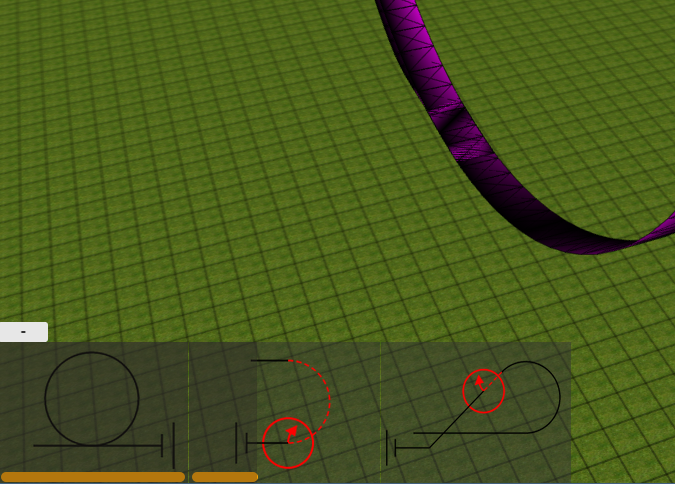
\includegraphics[width=1\textwidth]{images/movie.png}
  \caption{Movie reel overlaying the bottom of the canvas, with some figures loaded after the user typed in a string of OLAN.}
  \label{fig:vectors}
\end{figure}

Figure~\ref{fig:movie} also shows the animation progress, which was achieved by simply getting the current value of time which was used earlier in the 'getPointAt' method, then getting the percentage of this for the amount of moves entered. After this, a simple div was placed again using Jquery over the width of that percentage to achieve a darker coloured semi-transparent status bar. During tests of this feature (usability), one such issue was found that was caused when more than five manoeuvres were entered, the remaining Aresti figures were not present on the page, as it had been split into five sections. This means at this point of the project only the first five manoeuvres have their animation status shown. This is another feature that is hoped to be fixed before the end of the project implementation stage. 

\begin{table}[h]
\begin{tabular}{|l|l|l|l|p{7cm}|}
\hline
\textbf{Start} & \textbf{End} & \textbf{Duration} & \textbf{Progress} & \textbf{Comments}                                                                                                     \\ \hline
17-04-2015     & 19-04-2015   & 3 Days            & 50\%             &  Movie-reel implemented using images rather than constructing, though they show correctly the Aresti figures when the user enters OLAN. Issue found that requires fixing, concerning havign more than five manoeuvres availible on the reel.\\ \hline
20-04-2015     & 20-04-2015   & 1 Day            & 100\%             &  Usability tests complete, found the issue using them, and will test again once the issue is addressed.\\ \hline
\end{tabular}
\end{table}

\textbf{Feature overall progress: 75\%}

\subsubsection{Feature 10- Parameterisation of OLAN input}
The final feature that was added to the implementation Gantt chart was the one that would allow users to enter both parameters to OLAN notation (such as roll amount, length of entry and decent or others), and to tell the manouevre controller to move the start location of the next manoeuvre so many co-ordinates along the X or Y axis. Current progress on this feature after moving on in this stage of the project was that the second part functioned, allowing users to enter elements to move the start positon of the following maneouvres. However, as with some other features being implemented, it was felt that the time required to add the various prefixes and postfixes for each and every OLAN shape was too consuming on the overall project time. As with features where it was taking too long for specific parts, this will also be left in accordance with how the Gantt chart stands for time left for implementing and testing. The function for calculating the parameters was added besides the existing method taht reads input from the OLAN box, then creating vectors to create a path between a previous and next manoeuvre.

For the part of testing the half of the feature that worked, usability testing was the best approach here. In appendix D section~\ref{test:parameters} the test table can be found, and shows the feature passing for this aspect. By attempting to keep the workings of the application as similar as possible as to how OpenAreo handles parameters keeps consistancy for users across the web, and to keep consistancy in the OLAN language. While testing, it was found that the inut of the user should be heavily restricted and strictly typed, ensuring the user types the exact format that the paramaters should follow. After testing and evaluating the way that the OpenAero application handles this, it was decided the format should also be '(x,y)' where it is space seperated from other elements, and where x and y can be either negative or positive.

Following the completion of this particular parametersiation, the progress of the feature can now be reviewed.

\begin{table}[h]
\begin{tabular}{|l|l|l|l|p{7cm}|}
\hline
\textbf{Start} & \textbf{End} & \textbf{Duration} & \textbf{Progress} & \textbf{Comments}                                                                                                     \\ \hline
21-04-2015     & 23-04-2015   & 3 Days            & 50\%             &  Parameters for moving start positon of next manoeuvre ready, but individual OLAN maneouvre parameters not implemented yet.\\ \hline
24-04-2015     & 24-04-2015   & 1 Day            & 50\%             &  Can only test first half of the feature up to this point, will implement tests if second half if complete.\\ \hline
\end{tabular}
\end{table}

\textbf{Feature overall progress: 50\%}

\section{Final status and progress}
At this stage of the project, it is now possible to get a grasp of the overlal status of the application concerning implementation and testing. Using the progress reports from each feature, a general idea of the entire progress will combine all the completed features and then allow the creation of a brun-down chart to compare the current status with projected status. Although Burn-down charts are not FDD, it was chosen that the Scrum approach here would reveal more information around what work still needs to be completed, and when by. In order to create the burndown chart, the overall percentages of progress for each task should be collected. The list of features is shown in table~\ref{tbl:features}.

\begin{table}[h]
\centering
 \label{tbl:features}
\begin{tabular}{|l|l|l|l|l|}
\hline
\textbf{Feature} & \textbf{Start} & \textbf{End} & \textbf{Duration} & \textbf{Progress}                                                                                                \\ \hline
1 & 09-03-2015     & 11-03-2015   & 3 Days            & 100\%\\ \hline
2 & 12-03-2015     & 18-03-2015   & 7 Days            & 90\%\\ \hline
3 & 19-03-2015     & 20-03-2015   & 2 Days            & 100\% \\ \hline
4 & 21-03-2015     & 24-03-2015   & 4 Days            & 100\%\\ \hline
5 & 25-03-2015     & 08-04-2015   & 2 Weeks 2 Days    & 75\% \\ \hline
6 & 11-04-2015     & 09-04-2015   & 3 Days            & 100\% \\ \hline
7 & 12-04-2015     & 15-04-2015   & 5 Days            & 100\% \\ \hline
8 & 15-04-2015     & 16-04-2015   & 2 Days            & 100\% \\ \hline
9 & 17-04-2015     & 20-04-2015   & 4 Days            & 75\% \\ \hline
10 & 21-04-2015     & 24-04-2015   & 4 Days            & 50\% \\ \hline
\end{tabular}
\caption{Collected statuses of all features required, with their duration and percentage complete. Note: the dates shown the task was completed working on also include time done testing, and writing this stage of the report.}
\end{table}

Therefore, using the above table with dates of completion, a burndown chart up to this point can be created. The chart in figure~\ref{fig:burndown} shows the amount of features predicted remaining to implement versus the amount remaining at this time in the project. 

\begin{figure}[h]
  \centering
      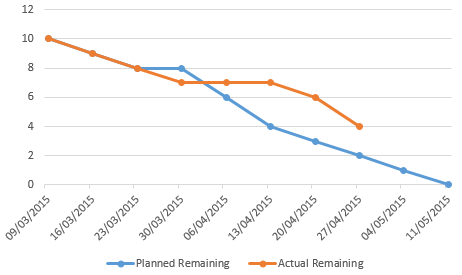
\includegraphics[width=0.8\textwidth]{images/burndown.png}
  \caption{Burndown chart of features implemented and tested fully. X axis represents number of features to implement, whilst Y axis shows the date that the features have been implemented by.}
  \label{fig:burndown}
\end{figure}

Although work appears to be behind schedule here, it should be noted that there is still both time remaining and some features are more than half complete. For strict purposes though and following the FDD manifesto, a feature can not be said to be complete until it is 100\% complete. 

Analysing the graph further, the main problem can be seen where work was halted on feature five, the creation of manoeuvres on the canvas. Becuase issues prolonged work here, it meant other features were pushed back until it was decided that they should be completed in order to make a more whole application. Due to moving onto and completing other features first alongside writing this part of the report, considerable time has been made up. The time remaining will now allow for any completion of features that are most important, and also fixes to others if possible. 

\subsection{After-test fixes and developments}

%fix OLAN, smoke trails too!
%hide movie reel
%fix reel scroll
%parameters OLAN not done
%check if manoeuvres fit

\section{User testing}
Now that the alocated time for implemntation and testing has been used, testing to see how the application meets its initial requirements is important. Along with the JSUnit tests and the usability tetsts that were created, user testing is a means of testing ideal for front-end applications where the usability of the application is paramount. There are a few routes that can be taken to perform user testing, one of which is a questionnaire. Rather than allowing the user to sedn feedback through suggestions or pros and cons, a quicker and more direct way to check the applicatins fulfills its needs is to provide the user with a set of direct questions, allowing them to state if they agree or dissagree. One example could be whether the colour scheme is sutible. By getting the amount agreeing above a certain threshold percentage wise would help show that the colour scheme aspect was correctly applied.

The questionnaire, which can be found in the appendices under appendix D, section~\ref{test:questionnaire} provided ten agree or dissagree questions that the users had to answer. Upon creating the questionnaire, these were then handed to a pick of 10 users, in technical and none-technical backgrounds to ensure a good spread of opinion. If just technical users were chosen, they might not see the application from the aspect of GUI as much as a standard user, as some users may find it harder to find things on a page. Things such as menus for instance may not be as visible and easy to find for users who have not seen similar layouts in the past, and it is important that they application has a level of being self-documenting.

The users selected to perform the testing comprised of eight students and two none-students. It was also ensured that half the students selected were not on a computer science related degree to ensure a wider set of technological knowledge. For each test, a brief description of the application was given to the user explaining the purpose and requiurements of the project and application, followed by the user trying out different features in the GUI and canvas. 

The questionnaires handed out were created using google forms, to keep the process on the internet fo easier tracking. Becuase this form of testing was not planned out originally on the Gantt chart at the start of this project, it was important that the tests were carried out as quickly as possible, so google forms were sent out and asked they could be returned a couple of days later. Indeed all ten questionnaires were returned, each of which all answers had been answered. This was very successful, as it then allowed the results to be analysed properly, and graphs created.

The results of each question can be found in appendix D section~\ref{test:questions}. Looking at the results, it can be assumed that... %TODOOOOOOOOOOOOOOOOOOOOOOOOOOOOO

\section{Implementation and testing review}
On completion of the process of the tests of the final application, a short review of
\chapter{Evaluation}
Upon completion of the application, it is now nessecary to evaluate both the application and project as a whole. This section will consider a number of 

%Examiners expect to find in your dissertation a section addressing such questions as:

%\begin{itemize}
 %  \item Were the requirements correctly identified? 
  % \item Were the design decisions correct?
   %\item Could a more suitable set of tools have been chosen?
   %\item How well did the software meet the needs of those who were expecting to use it?
   %\item How well were any other project aims achieved?
   %\item If you were starting again, what would you do differently?
%\end{itemize}

%Such material is regarded as an important part of the dissertation; it should demonstrate that you are capable not only of carrying out a piece of work but also of thinking critically about how you did it and how you might have done it better. This is seen as an important part of an honours degree. There will be good things and room for improvement with any project. As you write this section, identify and discuss the parts of the work that went well and also consider ways in which the work could be improved. Review the discussion on the Evaluation section from the lectures. A recording is available on Blackboard. 
% add any additional chapters here

\setemptyheader
\addcontentsline{toc}{chapter}{Appendices}
\chapter*{Appendices}
\pagebreak

% start the appendix - sets up different numbering
\fancypagestyle{plain}{%
%\fancyhf{} % clear all header and footer fields
\fancyhead[L]{\textsl{Appendix\ \thechapter}}
\fancyhead[R]{\textsl{\leftmark}}}

\appendix
\fancyhead[L]{\textsl{Appendix\ \thechapter}}
\fancyhead[R]{\textsl{\leftmark}}
\fancyhead[C]{}
\fancyfoot[C]{\thepage}
\renewcommand{\headrulewidth}{0.4pt}
\renewcommand{\chaptermark}[1]{\markboth{#1}{}}

\fancyhead[L]{\textsl{Appendix\ \thechapter}}
\fancyhead[R]{\textsl{\leftmark}}
\fancyfoot[C]{{\thepage} of \pageref{LastPage}}

% include any appendices here
\chapter{Background research and analysis}

\begin{landscape}
\section{Initial project Gantt chart}
\label{app:gantt1}
\begin{figure}[h!]
  \centering
   	\caption{Initial gantt chart, outline times throughout project activities, to be updated as time passes during the project span.}
      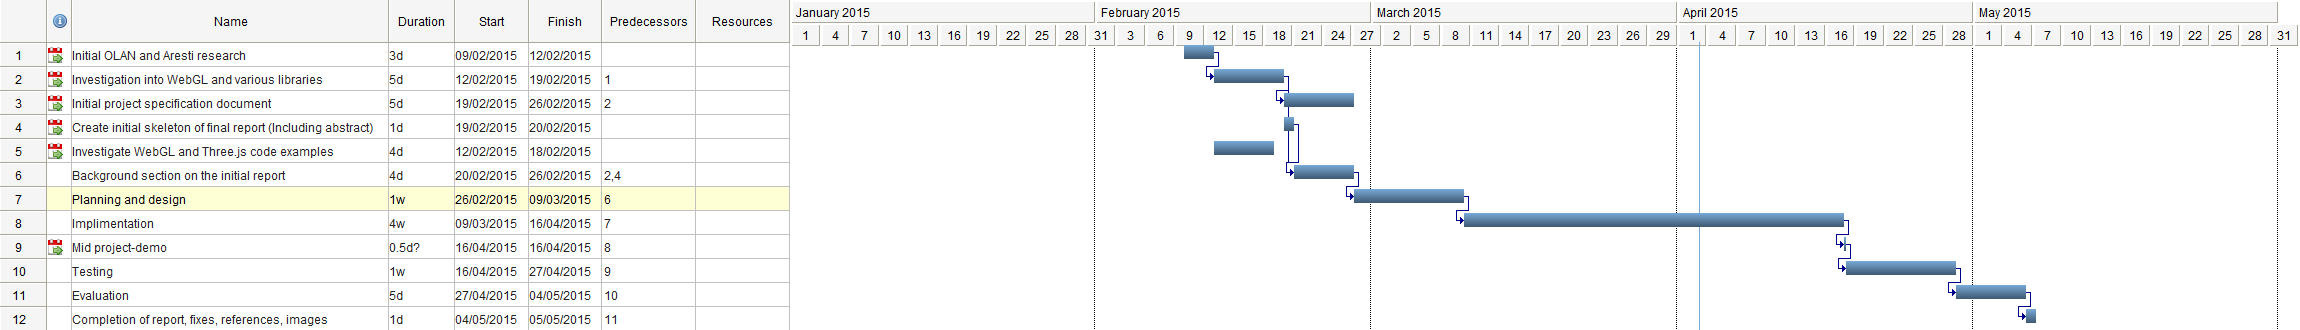
\includegraphics[width=23cm, height=6cm]{images/first.png}
\end{figure}
\end{landscape}
\clearpage

\section{Inital requirements analysis}
\label{app:init}
\begin{figure}[h!]
	\caption{Requirements brief created before a meeting to clarify questions on the initial requirements. The pdf continues onto the next page.}
	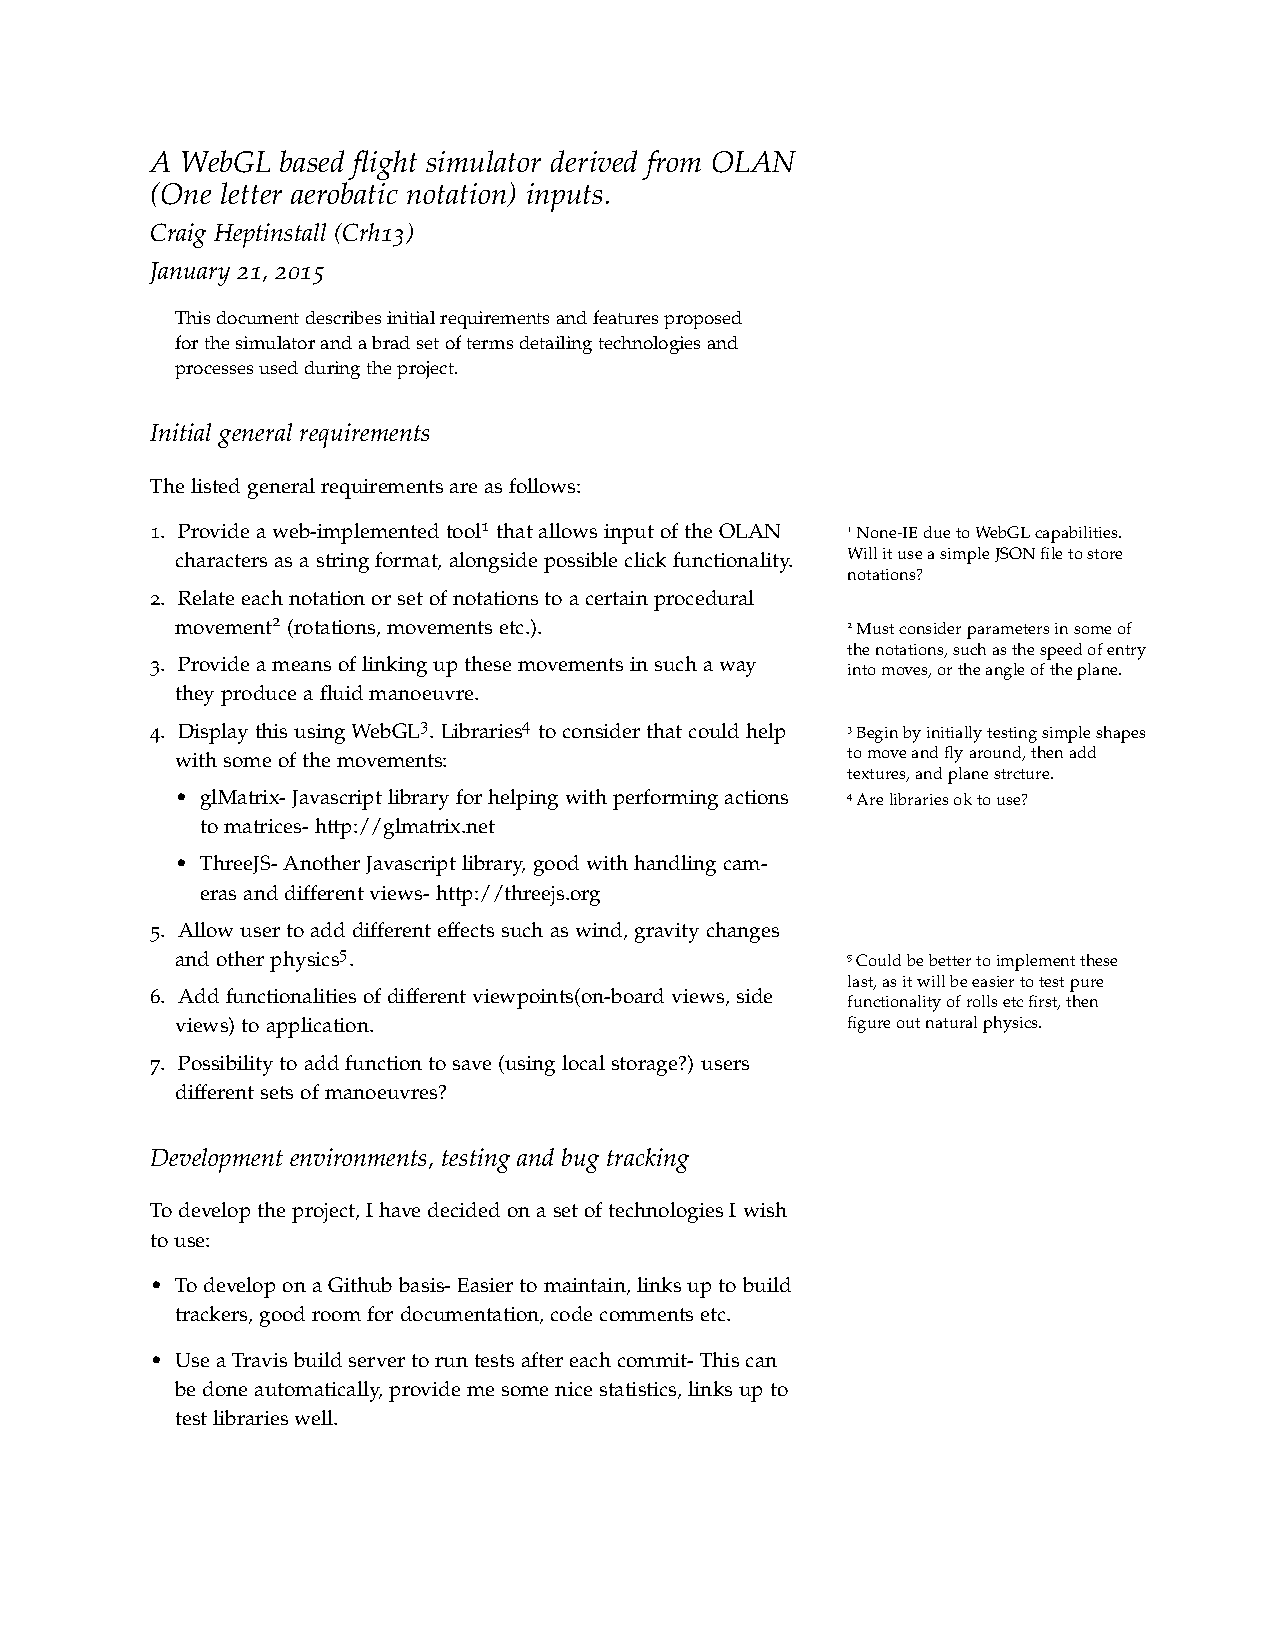
\includegraphics[width=18cm,height=18cm,page=1]{images/init.pdf}
\end{figure}

\begin{figure}[h!]
	\includegraphics[width=18cm,height=18cm,page=2]{images/init.pdf}
\end{figure}
\clearpage

\section{OLAN understandings}
\label{app:olan}
\begin{figure}[h!]
	\centering
	\caption{A document created before a second meeting, outlining my current undertsanding of the OLAN language, and how manoeuvres can be constructed from smaller single-element ones.}
	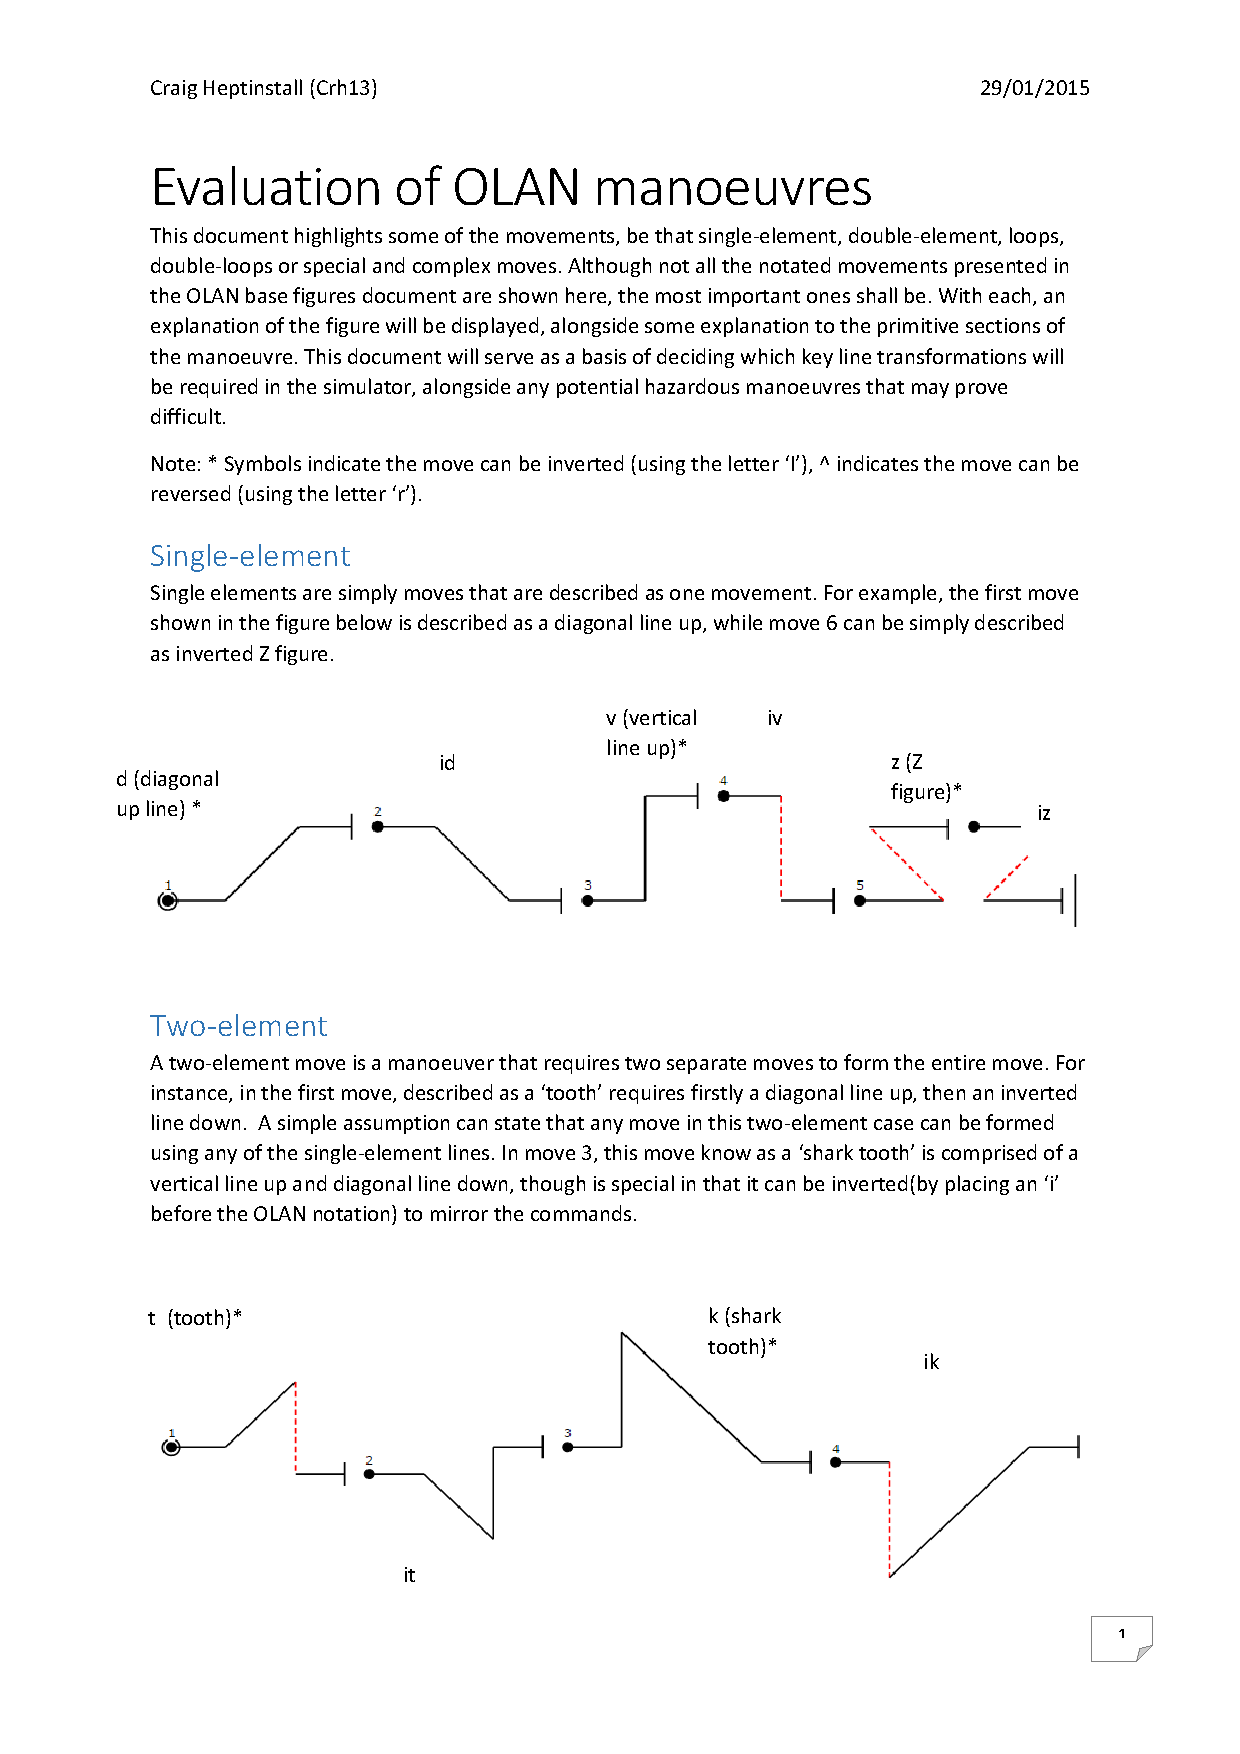
\includegraphics[width=16cm,height=20cm,page=1]{images/eval.pdf}
\end{figure}
\begin{figure}[h!]
	\centering
	\includegraphics[width=16cm,height=21cm,page=2]{images/eval.pdf}
\end{figure}
\begin{figure}[h!]
	\centering
	\includegraphics[width=16cm,height=21cm,page=3]{images/eval.pdf}
\end{figure}
\begin{figure}[h!]
	\centering
	\includegraphics[width=16cm,height=21cm,page=4]{images/eval.pdf}
\end{figure}
\begin{figure}[h!]
	\centering
	\includegraphics[width=16cm,height=21cm,page=5]{images/eval.pdf}
\end{figure}

\clearpage

\begin{landscape}
\section{Revised FDD Gantt chart}
\label{app:gantt2}
\begin{figure}[h!]
  \centering
  	\caption{More detailed Gantt chart, focuses on the implimentation and testing stratedgy of each feature. As you can see, prioritised tasks are the first to be completed.}
      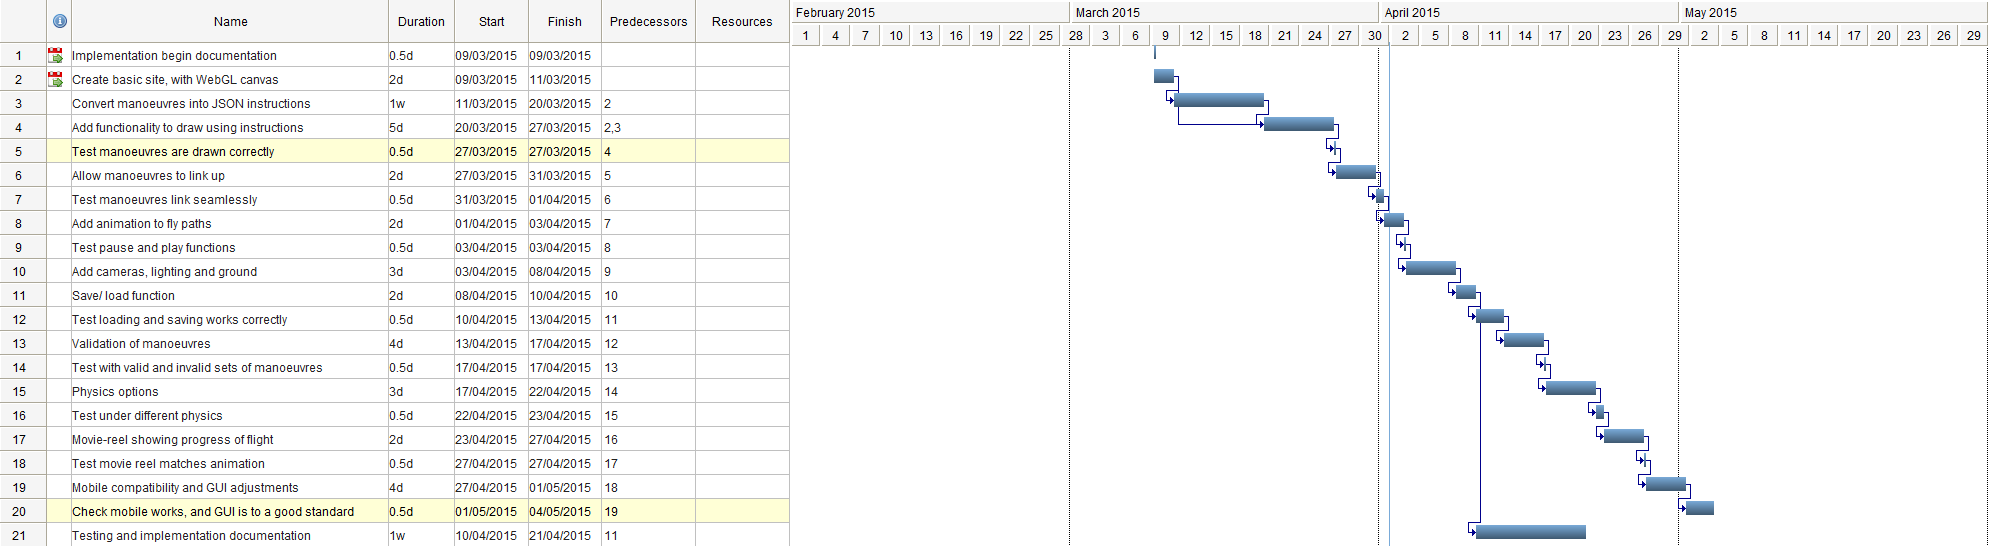
\includegraphics[width=23cm, height=6cm]{images/second.png}
\end{figure}
\end{landscape}
\clearpage
\chapter{Third-Party Code, Libraries and tools}
There are some libraries and tools that were used during the project to design and implement the application. The libraries mentioned here have a description of what they are, why they were used in my the application, and links to both the library home page and library license. In addition to this, a few tools that were used behind the scenes of this project have been mentioned. 

\textbf{Three.js} - This project has been used to handle all the WebGL features of the application, providing methods to access the shader code and handle any animations. From loading up models to creating cameras, this library was used extensively through the project. Available on the three.js site \cite{ThreeJs}, licensed under MIT \cite{MIT}.

\textbf{StatsJs} - A library for monitoring performance of JavaScript code. This was used to see how well my code was performing in relation to frames per second. The library places a FPS counter onto the page, and helped monitor how different effects can reduce performance. Available on the Javascripttoo page \cite{stats}, licensed under MIT \cite{MIT}.

\textbf{JQuery} - A library for interacting with both HTML and some back end methods. This library was used for support of RequireJS, foundation CSS and used for connecting the back end of the application with the GUI. Licensed under MIT \cite{MIT}, currently available from the JQuery site \cite{JQuery}.

\textbf{Foundation} - A CSS framework used to help build a responsive site. Similar to the bootstrap library, it comes with lots of pre-styled classes, so it made building the site a matter of created nested div tags. Currently availible from the foundation page \cite{foundation}, licensed under MIT \cite{MIT}.

\textbf{RequireJS} - A framework for creating modulation of JavaScript code. Used to modulate the application, and dynamically load up JavaScript files defined in each module. Dual licensed under MIT \cite{MIT} and BSD \cite{BSD}, require is available from the RequireJS site \cite{requirejs}.

Alongside the libraries mentioned above, there were some tools which helped form this report. Mainly diagram creators, they helped in the creation of supporting illustrations.

\textbf{Gantter} - A an on-line application allowing the creation of Gantt charts, with export capabilities. This was used to create both Gantt charts present in this report.

\textbf{Creatly} - On-line diagram creation tool for projects. Used to create all use-cases, class diagram, flow charts and MVC diagrams, this proved a handy tool throughout design.

\textbf{Mockflow} - An on-line application for the designing of wire-frames. Allowed me to draw and style mock ups of the site before creating it. Had a very useful feature which allowed me to export the mock up to HTML code, instantly creating the site.

\textbf{TeXcount} - \LaTeX word counter used to keep check on the amount of words in the report. Available as a Perl script as well as on-line.

\chapter{Code samples}

\section{Off-canvas HTML code, showing how menus are hidden }
\label{code:canvas}
\begin{figure}[h!]
\caption{HTML code showing the page is divided into two, one for the canvas, and one for the menu. The 'off-canvas-list' has sub menus that allow more menus to be hidden to the left.}
\begin{lstlisting}
 <div class="off-canvas-wrap" data-offcanvas>
    <div class="inner-wrap">
        <aside class="left-off-canvas-menu">
            <ul class="off-canvas-list">
                <li>
                    <label>Option Categories</label>
                </li>
                <li class="has-submenu">
                    <li class="has-submenu">
                        <a href="#">OLAN</a>
                    </li>
                    <li class="has-submenu">
                        <a href="#">Physics</a>
                    </li>
                    <li class="has-submenu">
                        <a href="#">Save/Load</a>
                    </li>
                </li>
            </ul>
            <footer id="footer" class="row">
            </footer>
        </aside>
        <div id="container">
            
        </div>
        <a class="exit-off-canvas"></a>
    </div>
</div>
\end{lstlisting}
\end{figure}

\section{JSON OLAN instructions example}
\label{code:jsonmoves}
\begin{figure}[h!]
\caption{JSON code showing a vertical upline defined by JSON instructions.}
\begin{lstlisting}
 {
            "variant": [{
                "component": [{
                    "_pitch": "NIL",
                    "_roll": "NIL",
                    "_yaw": "NIL",
                    "_length": "10"
                },
                {
                    "_pitch": "POS",
                    "_roll": "NIL",
                    "_yaw": "NIL",
                    "_length": "1"
                } ,
                {
                    "_pitch": "POS",
                    "_roll": "NIL",
                    "_yaw": "NIL",
                    "_length": "1"
                }],
                "_olanPrefix": "",
                "_name": "Vertical up line"
            }],
            "_olan": "q"
        },
\end{lstlisting}
\end{figure}

\section{RequireJS setup code}
\label{code:requireJS}
\begin{figure}[h!]
\caption{Snippet of code showing how RequireJS starts the application. The RequireJS library is loaded onto the page, the configuration telling the library the base of the application JavaScript files is set, and then is told to start by running the main.js file.}
\begin{lstlisting}
<script>
    require.config({
        baseUrl: 'js',
    });
    require(["main"]);
</script>
\end{lstlisting}
\end{figure}

\clearpage

\section{Converting JSON representations into vectors}
\label{code:jsonmovesJS}
\begin{figure}[h!]
\caption{Snippet of code responsible for converting the manoeuvre objects into vectors, allowing the creation of Three.js spline curves.}
\begin{lstlisting}
for (m in values) {

    var components = values[m]["components"];

    for (var i = 0; i < components.length; i++) {
        var component = components[i];
        var prevVector = new THREE.Vector3(0, 0, 0);

        if (linePoints.length > 0)
            prevVector.copy(linePoints[linePoints.length - 1]);

        if (component.PITCH == 0 && component.YAW == 0 && component.ROLL == 0) {
            prevVector.setZ(prevVector.z + (component.LENGTH * 10));
            linePoints.push(prevVector);
        } else {
            var axis = new THREE.Vector3(1, 0, 0);
            var angle = Math.PI / 180 * angleDiv * -component.PITCH;
            prevVector.applyAxisAngle(axis, angle);

            var axis = new THREE.Vector3(0, 1, 0);
            var angle = Math.PI / 180 * angleDiv * component.YAW;
            prevVector.applyAxisAngle(axis, angle);

            prevVector.setZ(prevVector.z + (component.LENGTH * 10));
            linePoints.push(prevVector);
        }
    }
    var startVector = new THREE.Vector3(0, 0, 0);
    startVector.copy(prevVector);
    linePoints.push(startVector);
}
\end{lstlisting}
\end{figure}

\section{Using local storage to export scenarios}
\label{code:localStorage}
\begin{figure}[h!]
\caption{Code used for checking local storage compatibility.}
\begin{lstlisting}
exportToLocalStorage: function(manoeuvres) {
    if (checkLocalStoragePermitted()) {
        if (!localStorage.getItem("autoLoad"))
            return;
        // Store
        localStorage.setItem("manoeuvres", manoeuvres);
    }
}
\end{lstlisting}
\end{figure}
\chapter{Application tests}

\section{Usability testing for the GUI front-end}
\label{test:canvas}
\begin{table}[h]
\begin{tabular}{|p{4.5cm}|p{4.5cm}|p{2cm}|p{2.5cm}|}
\hline
\textbf{Test} & \textbf{Pred. Result} & \textbf{Pass/ Fail} & \textbf{Comment}                        \\ \hline
Open menu    &   Menu is displayed on the left, canvas moves right. &  Pass          &    \\ \hline
Close menu    &   Menu hides to the left, canvas is pulled back in to fill page. &   Pass         &     \\ \hline
Resize window to mobile size    & Menu changes to mobile view, canvas still fills page.   & Pass           &     \\ \hline
Open mobile menu    & Menu displaying OLAN input, about and help pages listed.   &     Pass       &     \\ \hline
Open help page    &  Overlay appears from above, covers canvas with white box and text.  &       Pass     &     \\ \hline
Open about page    &  Overlay appears from above, covers canvas with white box and text.  &      Pass      &     \\ \hline
Close about page    &  Box fades away.  &      Pass      &     \\ \hline
Open sub-menu    &  Menu pulls in from left in side to cover current menu. Shows options of certain menu chosen.  &    Pass        &     \\ \hline
Click back on sub-menu    &  Sub-menu slides to left and reveals original top level menu.  &    Pass        &     \\ \hline
\end{tabular}
\caption{Usability test table for testing the GUI.}
\end{table}

\clearpage

\section{Test utility code for creating GUI before testing}
\label{test:utils}
\begin{figure}[h!]
\caption{RequireJS module for allowing test units to share methods providing them with GUI elements before tests. Tear down code removes the elements after each test.}
\begin{lstlisting}
define(function(){ 
	return {
		setUpAppend: function(toAppend) {
		            toAppend = "<div id='added'>" + toAppend + "</div>";
		            $('body').append(toAppend);
		},
        removeAppended: function(){
            $("#added").remove();
        }
	}
});
\end{lstlisting}
\end{figure}

\section{Test Unit code for converting JSON to manoeuvre instruction object}
\label{test:jsonmvoes}
\begin{figure}[h!]
\caption{JSUnit code created to test the capabilites of changing the JSON instructions into objects.}
\begin{lstlisting}
\end{lstlisting}
\end{figure}

\section{Test Unit code for checking lights and ground are created successfully}
\label{test:lights}
\begin{figure}[h!]
\caption{Checks if objects for both are created at runtime of the application.}
\begin{lstlisting}
\end{lstlisting}
\end{figure}

\section{Usability testing for cameras}
\label{test:cameras}
\begin{table}[h]
\begin{tabular}{|p{4.5cm}|p{4.5cm}|p{1cm}|p{4cm}|}
\hline
\textbf{Test} & \textbf{Pred. Result} & \textbf{Pass/ Fail} & \textbf{Comment}                        \\ \hline
Test drag mouse to rotate around canvas    &  Camera should rotate around the scene.  &     Fail       &  Changed after fail, due to camera rotation around the point(0,0,0). Changed now so that it rotates around current camera location.    \\ \hline
Scroll zoom in    &   Camera should focus in on the center of the canvas. &   Pass         &    \\ \hline
Scroll zoom out    &   Camera should see more of the canvas as mouse scrolls out. & Pass           &     \\ \hline
Left keyboard key to move left    &  Camera moves 10px to the left.  &   Pass         &     \\ \hline
Right keyboard key to move right    & Camera moves 10px to the right.   &    Pass        &     \\ \hline
Up keyboard key to move forward    &  Camera moves 10px forward its Z axis.  &   Pass         &     \\ \hline
Down keyboard key to move backwards    &  Camera moves 10px backwards its Z axis.  &  Pass          &     \\ \hline
Switch to onboard camera view   &  Camera changes to 0,0,0 looking ahead. &  Pass          &     \\ \hline
\end{tabular}
\caption{Tests various actions from the user to do with both cameras.}
\end{table}

\section{Test Unit code for animation controller getters and setters}
\label{test:animation}
\begin{figure}[h!]
\caption{Unit code checking information is set correctly, and if it can be changed at stored for various animation properties.}
\begin{lstlisting}
\end{lstlisting}
\end{figure}

\section{Test Unit code for checking import and export to JSON/ local storage functionality}
\label{test:save}
\begin{figure}[h!]
\caption{JSUnit code for checking flight paths export correctly to JSON and local storage, and check importing back works.}
\begin{lstlisting}
\end{lstlisting}
\end{figure}

\section{Usability testing for GUI options}
\label{test:options}
\begin{table}[h]
\begin{tabular}{|p{4.5cm}|p{4.5cm}|p{2cm}|p{2.5cm}|}
\hline
\textbf{Test} & \textbf{Pred. Result} & \textbf{Pass/ Fail} & \textbf{Comment}                        \\ \hline
Type OLAN into input box to create figures    &  Loop should appear when 'o' is typed in, and movie-reel should show manouvre at bottom.  &            &     \\ \hline
Use dropdown in OLAN options to add a figure    &  Loop should be added to canvas when chosen from dropdown.  &     Pass       &     \\ \hline
Increase and decrease scale    &  Figures on canvas should become bigger or smaller depending on scale.  &       Pass     &     \\ \hline
Increase and decrease extrusion segments    &  Curves should become less and more smooth depending on extrusion.  &       Pass     &     \\ \hline
Increase and decrease radius    &  More sides to the figure should appear the higher the radius.  &     Pass       &     \\ \hline
Increase animation speed    &   Speed of flight should increase depending on slider of speed. &            &     \\ \hline
Turn switch on for auto repeat of animation    &  When on, when animating, should loop from beginning to end endlessly.  &       Pass     &     \\ \hline
Switch auto save on and close application, then re-open    &  When on, if application is closed and re-opened then routines should be added automatically. Vice versa.  &       Pass     &     \\ \hline
Export to JSON using button    &  JSON file begins to download on click.  &      Pass      &     \\ \hline
Import JSON file using file chooser  &  Routine should load up when selecting a file.  &      Pass      &     \\ \hline
\end{tabular}
\caption{Usability test table for user interface options, including OLAN entry box, OLAN dropdown, pyhsics options, animation options and exporting/ importing to JSON.}
\end{table}

\section{Usability testing providing parameters between OLAN}
\label{test:parameters}
\begin{table}[h]
\begin{tabular}{|p{4.5cm}|p{4.5cm}|p{2cm}|p{2.5cm}|}
\hline
\textbf{Test} & \textbf{Pred. Result} & \textbf{Pass/ Fail} & \textbf{Comment}                        \\ \hline
Enter empty parameters '()'    &  No change to start location of next manoeuvre should occur.  &     Pass       &     \\ \hline
Empty correct format paramaters '(10,10)'    &  Should move start of next manoeuvre 10 pixels up, 10 to the left.  &      Pass      &     \\ \hline
Enter parameters without space between OLAN    & The manouvre nor parameters will be placed on the canvas.   &        Pass    &     \\ \hline
Enter parameters with negative values '(-10,-10)'    &  Should move start of next manoeuvre 10 pixels down, 10 to the right.  &       Pass     &     \\ \hline
Enter parameters on a manoeuvre "o''"  &  Loop should be drawn with three times the length exit travel.  &        Fail    &   Parameter had np effect to the loops exit, and prevented the manouvre from being drawn.  \\ \hline
\end{tabular}
\caption{Usability test table showing results of typing in parameters alongside maneouvres.}
\end{table}

\clearpage

\section{User questionnaire}
\label{test:questionnaire}
\begin{figure}[h!]
    \caption{A google forms questionnaire created to allow users to give feedback about the application.}
    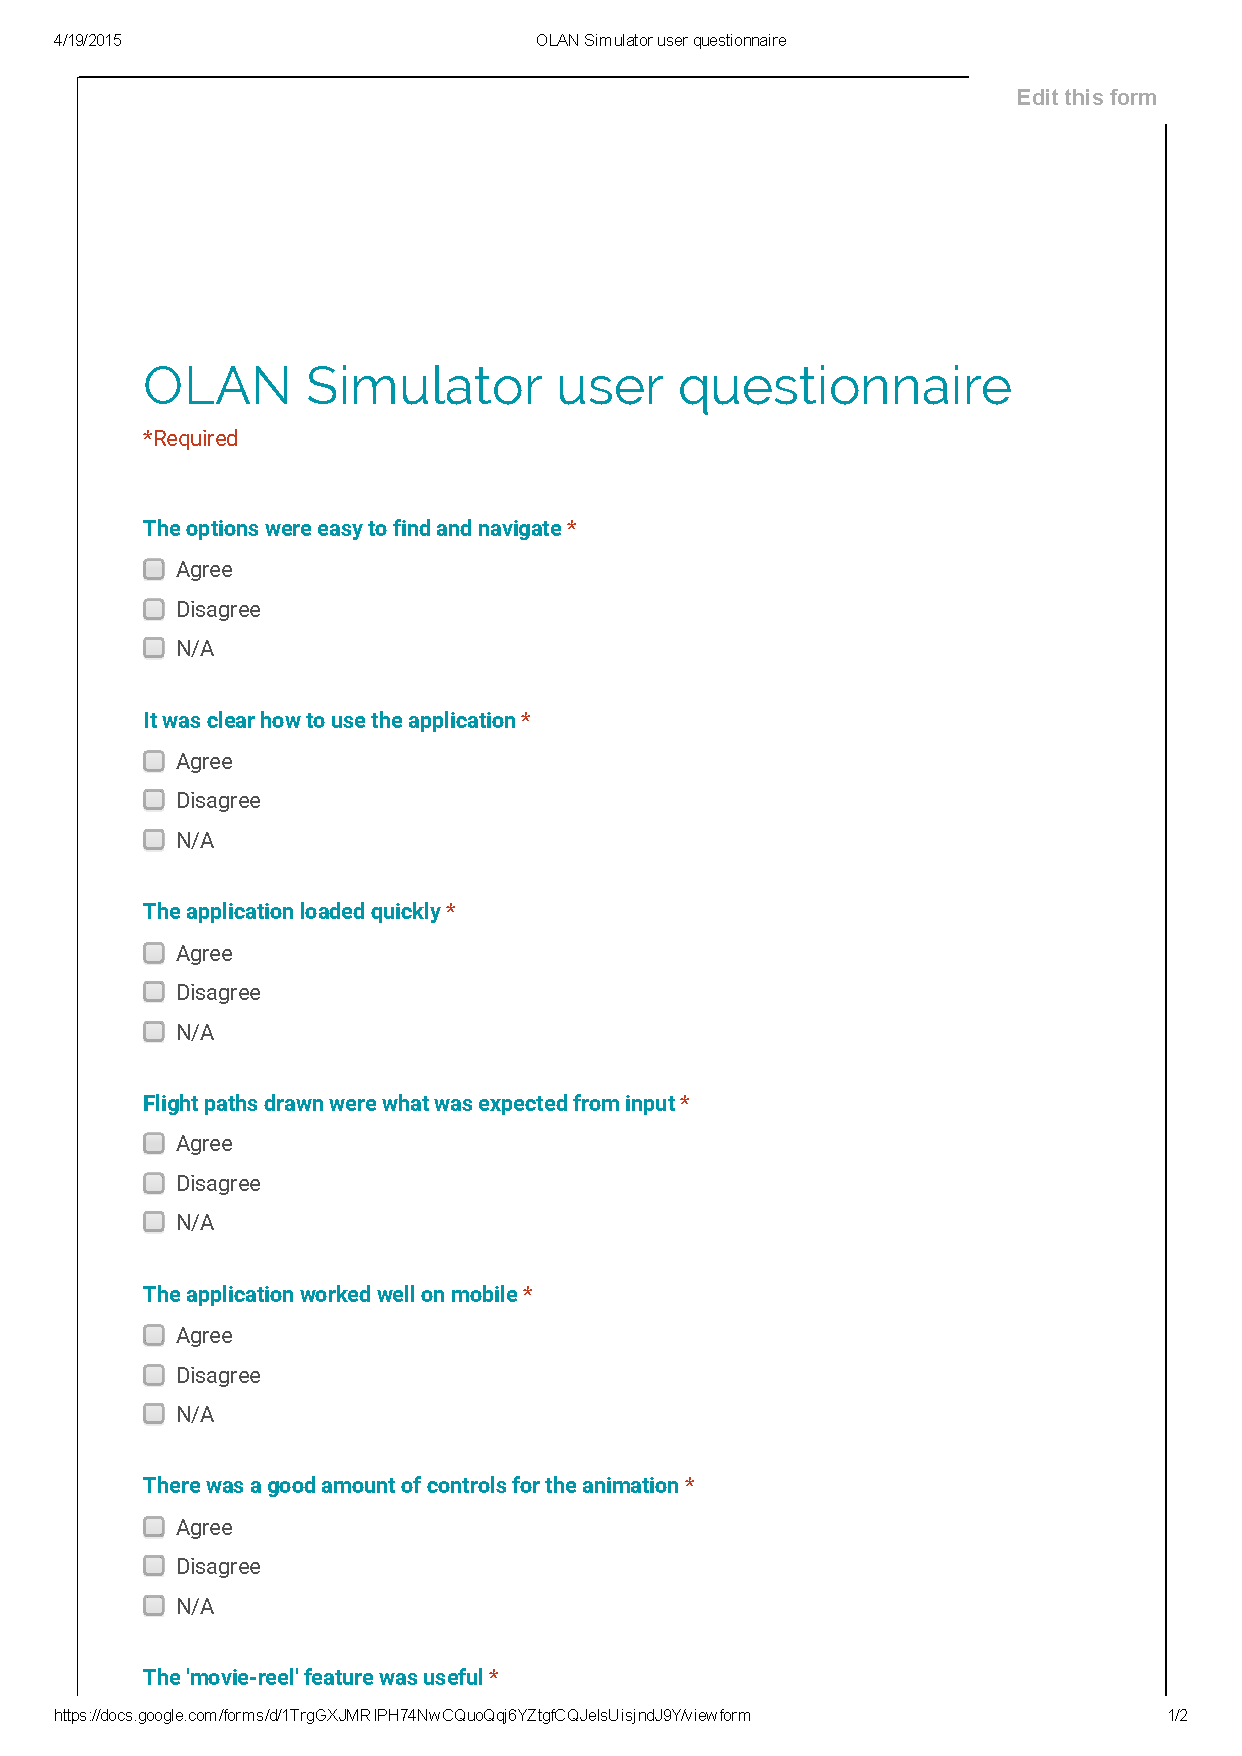
\includegraphics[width=15cm,height=18cm,page=1]{images/questionnaire.pdf}
\end{figure}

\begin{figure}[h!]
    \includegraphics[width=15cm,height=18cm,page=2]{images/questionnaire.pdf}
\end{figure}

\clearpage

\section{User questionnaire results}
\label{test:questionnaireResults}
\begin{figure}[h!]
    \caption{Statistics from the questionnaire results, showing percentages of answers and comments/ suggestions.}
    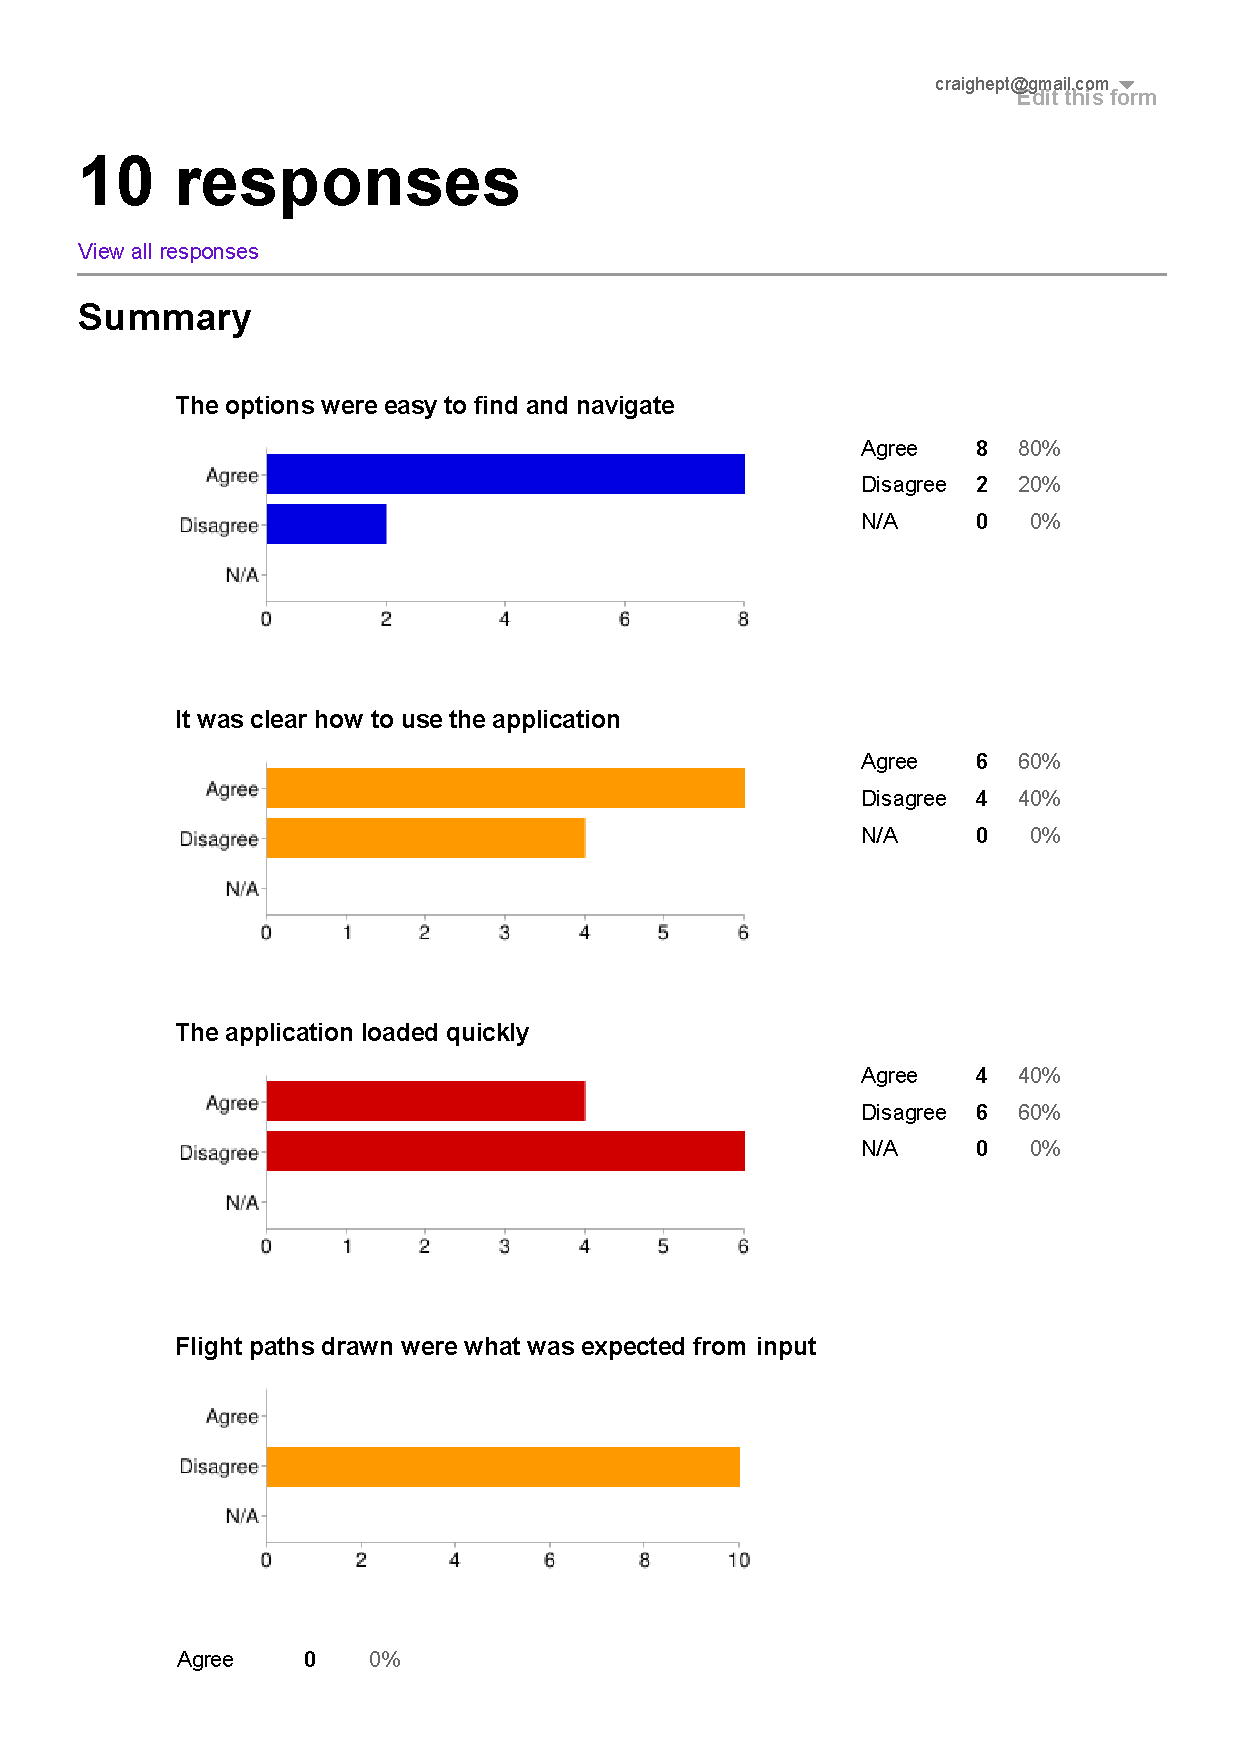
\includegraphics[width=15cm,height=18cm,page=1]{images/questionnaireResults.pdf}
\end{figure}

\begin{figure}[h!]
    \includegraphics[width=15cm,height=18cm,page=2]{images/questionnaireResults.pdf}
\end{figure}

\begin{figure}[h!]
    \includegraphics[width=15cm,height=18cm,page=3]{images/questionnaireResults.pdf}
\end{figure}
\chapter{Post-Report changes}

See any appended pages following this for changes done to code after this report was printed and binded. 2 Pages have been allocated, therefore blank pages will be present if both are not used.

\clearpage

\section{Resulted and on-going work}
When this report was printed, there was still the issue present with some of the OLAN manoeuvres. The main issue included the odd behavior of when a new manoeuvre was added, the rotation and thus places where vectors where being added seemed to be out of place to the same distance of how far the manoeuvre started in comparison to the start of the first manoeuvre. Although every effort was taken to attempt to resolve this issue, the application still faces this issue. Following various searches through question/ answer site like 'Stackoverflow', conversations with people who have had experience using the Three.js library and even direct questions on the Github repository with the Three.js developers, it was decided that the issue would take too long and too much restructuring of the current application to create a viable fix. \\

Furthering the suggested ideas mentioned in the implementation part of this report, the way that vectors were rotated were changed from using a matrices to a Euler. The reason for this was that Three.js handled the matrix automatically, increasing the speed it is done in. It was also though that this means of rotation of vectors might have fixed the issue above, though this too did not work. \\

Although the primary issue was never completed in time for the project hand-in, it was ensured that both the JSDoc and refactoring was completed before the end of project. This included adding relevant comments for any new methods created during refactoring, alongside changing current documentation where method existence reasons changed. In addition to this, a read-me file was added to the source code folder, to ensure that any persons that may want to run the application themselves, or edit the application for their own use know how to properly set it up and edit it correctly. A final change performed was creating a general source folder clean up, including deleting unused library classes, and renaming both folders a files in a way that followed a universal standard. Touch ups to the GUI was also added, such as mouse hides on the canvas after a few seconds while animations occur, and checks done to ensure users who try use the application without a WebGL enabled browser are notified.

Overall, although the issue was never fixed in the timescale given, it was a thoroughly enjoyed project to the very end of available time, and because of this not only will the issue be attempted to be fixed, but it will be an application that is developed over the coming months or even years as a hobby. Using time correctly for potential issues as the one experienced in this project will be taken into account for future work, and it will be ensured that considerations and actions are taken faster (e.g. changing library altogether for a solution, though this project was too far in.)

\clearpage

\newpage\mbox{}\newpage

\fancypagestyle{plain}{%
   \fancyhead{} %[C]{Annotated Bibliography}
   \fancyfoot[C]{{\thepage} of \pageref{LastPage}} % except the center
   \renewcommand{\headrulewidth}{0pt}
   \renewcommand{\footrulewidth}{0pt}
}

\setemptyheader

\nocite{*} % include everything from the bibliography, irrespective of whether it has been referenced.

% the following line is included so that the bibliography is also shown in the table of contents. There is the possibility that this is added to the previous page for the bibliography. To address this, a newline is added so that it appears on the first page for the bibliography. 
\addcontentsline{toc}{chapter}{Annotated Bibliography} % Adds References to contents page

%
% example of including an annotated bibliography. The current style is an author date one. If you want to change, comment out the line and uncomment the subsequent line. You should also modify the packages included at the top (see the notes earlier in the file) and then trash your aux files and re-run. 
%\bibliographystyle{authordate2annot}
\bibliographystyle{IEEEannot}
\renewcommand{\bibname}{Annotated Bibliography} 
\bibliography{References/references} % References file


\end{document}
